\documentclass[degree=bachelor, tocarialchapter]{thuthesis}
% 选项
%   degree=[bachelor|master|doctor|postdoctor], % 必选,学位类型
%   secret,                % 可选(默认:关闭),是否有密级
%   tocarialchapter,       % 可选(默认:关闭),章目录中使用黑体(这项表示同时打开下面两项)
%   tocarialchapterentry,  % 可选(默认:关闭),单独控制章标题在目录中使用黑体
%   tocarialchapterpage,   % 可选(默认:关闭),单独控制章页码在目录中使用黑体
%   pifootnote,            % 可选(默认:关闭),页脚编号采用 pifont 字体符号,建议打开

% 所有其它可能用到的包都统一放到这里了,可以根据自己的实际添加或者删除。
\usepackage{thuthesis}

% 定义所有的图片文件在 figures 子目录下
\graphicspath{{figures/}}

% 可以在这里修改配置文件中的定义。导言区可以使用中文。
% \def\myname{薛瑞尼}

\begin{document}

%%% 封面部分
\frontmatter
\thusetup{
  %******************************
  % 注意:
  %   1. 配置里面不要出现空行
  %   2. 不需要的配置信息可以删除
  %******************************
  %
  %=====
  % 秘级
  %=====
  secretlevel={秘密},
  secretyear={10},
  %
  %=========
  % 中文信息
  %=========
  ctitle={基于GST的超表面光学器件研究},
  cdegree={工学学士},
  cdepartment={电子工程系},
  cmajor={电子科学技术类},
  cauthor={白林禹},
  csupervisor={李洪涛$\ $副研究员},
 %  cassosupervisor={陈文光教授}, % 副指导老师
  % ccosupervisor={某某某教授}, % 联合指导老师
  % 日期自动使用当前时间,若需指定按如下方式修改:
  % cdate={超新星纪元},
  %
  % 博士后专有部分
  cfirstdiscipline={计算机科学与技术},
  cseconddiscipline={系统结构},
  postdoctordate={2009年7月——2011年7月},
  id={编号}, % 可以留空: id={},
  udc={UDC}, % 可以留空
  catalognumber={分类号}, % 可以留空
  %
  %=========
  % 英文信息
  %=========
  etitle={An Introduction to \LaTeX{} Thesis Template of Tsinghua University v\version},
  % 这块比较复杂,需要分情况讨论:
  % 1. 学术型硕士
  %    edegree:必须为Master of Arts或Master of Science(注意大小写)
  %             “哲学、文学、历史学、法学、教育学、艺术学门类,公共管理学科
  %              填写Master of Arts,其它填写Master of Science”
  %    emajor:“获得一级学科授权的学科填写一级学科名称,其它填写二级学科名称”
  % 2. 专业型硕士
  %    edegree:“填写专业学位英文名称全称”
  %    emajor:“工程硕士填写工程领域,其它专业学位不填写此项”
  % 3. 学术型博士
  %    edegree:Doctor of Philosophy(注意大小写)
  %    emajor:“获得一级学科授权的学科填写一级学科名称,其它填写二级学科名称”
  % 4. 专业型博士
  %    edegree:“填写专业学位英文名称全称”
  %    emajor:不填写此项
  edegree={Doctor of Engineering},
  emajor={Computer Science and Technology},
  eauthor={Xue Ruini},
  esupervisor={Professor Zheng Weimin},
  eassosupervisor={Chen Wenguang},
  % 日期自动生成,若需指定按如下方式修改:
  % edate={December, 2005}
  %
  % 关键词用“英文逗号”分割
  ckeywords={GST, 功能可调, 超表面},
  ekeywords={GST, adjustable function, metasurface}
}

% 定义中英文摘要和关键字
\begin{cabstract}
超表面光学器件可以在小于波长的厚度尺寸下实现传统光学器件的功能,如聚焦、分光、起偏等,具有重要的理论意义和应用前景。但是超表面光学器件一旦被制作出来,其功能就固定了,无法根据需要变化。寻求一种功能可调的超表面光学器件设计和制作方法是当前研究的一个热点。

本论文针对基于GST材料的功能可调超表面光学器件开展研究。

首先,本论文对二维排布的GST纳米柱阵列进行了仿真。结果表明这种结构通过GST晶化状态的改变可以实现$\left ( 0, 2\pi \right )$的相位变化,从而可以被用于制作功能可调的超表面光学器件。

其次,本论文优化了GST薄膜材料的磁控溅射制备参数。在0.5Pa的氩气氛围,80W溅射功率下溅射速率为$35\ nm \cdot{} min^{-1}$且制备得到的是表面平整的非晶化薄膜。

第三,本论文对GST薄膜相变前后的折射率、透过率随波长的变化进行了测试。结果表明非晶态的折射率为$\left ( 3.47 + 1.09i \right )$,晶化之后为$\left ( 7.74 + 3.49i \right )$。制得的GST薄膜样品对于波长在$1.4\ \mu m$以上的光有高透过率,波长在$1.1\ \mu m$以下的光有高反射率。

本文的研究成果为后续功能可调的超表面光学器件研究打下了坚实基础。
\end{cabstract}

% 如果习惯关键字跟在摘要文字后面,可以用直接命令来设置,如下:
% \ckeywords{\TeX, \LaTeX, CJK, 模板, 论文}

\begin{eabstract}
 Metasurface optical devices can realize the functions of traditional optical devices such as focusing, splitting, and polarizing at the thicknesses smaller than the wavelength, which have important theoretical significance and application prospects. However, once the metasurface optics are manufactured, their functions are fixed and cannot be changed as need. The search for a function-adjustable metasurface optical device design and fabrication method is a hot topic in current research.
This dissertation focuses on functionally adjustable super-surface optical devices based on GST materials.

First, this paper simulates a two-dimensional array of GST nanopillar arrays. The results show that this structure can achieve the phase change of $\left (0, 2\pi\right)$ through the change of the crystallization state of GST, which can be used to make a function-adjustable super-surface optical device.

Secondly, this paper optimized the magnetron sputtering preparation parameters of GST thin film materials. In an argon atmosphere of 0.5 Pa, the sputtering rate is $35 nm\cdot{}min^{-1}$ at a sputtering power of 80 W and an amorphized film with a flat surface is prepared.

Third, this paper tests the change of refractive index and transmittance of the GST film before and after phase transformation with wavelength. The result shows that the refractive index of the amorphous state is $\left (3.47 + 1.09i \right)$ and after crystallization is $\left (7.74 + 3.49i \right)$. The resulting GST thin film sample has a high transmittance for light at wavelengths above $1.4\ \mu m$, and high reflectance for light at wavelengths below $1.1\ \mu m$.

The research results of this paper lay a solid foundation for the follow-up function research of super-surface optical devices.
\end{eabstract}

% \ekeywords{\TeX, \LaTeX, CJK, template, thesis}

% 如果使用授权说明扫描页,将可选参数中指定为扫描得到的 PDF 文件名,例如:
% \makecover[scan-auth.pdf]
\makecover

%% 目录
\tableofcontents

%% 符号对照表
% \begin{denotation}[3cm]
\item[HPC] 高性能计算 (High Performance Computing)
\item[cluster] 集群
\item[Itanium] 安腾
\item[SMP] 对称多处理
\item[API] 应用程序编程接口
\item[PI] 聚酰亚胺
\item[MPI] 聚酰亚胺模型化合物,N-苯基邻苯酰亚胺
\item[PBI] 聚苯并咪唑
\item[MPBI] 聚苯并咪唑模型化合物,N-苯基苯并咪唑
\item[PY] 聚吡咙
\item[PMDA-BDA]	均苯四酸二酐与联苯四胺合成的聚吡咙薄膜
\item[$\Delta G$] 活化自由能 (Activation Free Energy)
\item[$\chi$] 传输系数 (Transmission Coefficient)
\item[$E$] 能量
\item[$m$] 质量
\item[$c$] 光速
\item[$P$] 概率
\item[$T$] 时间
\item[$v$] 速度
\item[劝学] 君子曰:学不可以已。青,取之于蓝,而青于蓝;冰,水为之,而寒于水。木
  直中绳。輮以为轮,其曲中规。虽有槁暴,不复挺者,輮使之然也。故木受绳则直,金就
  砺则利,君子博学而日参省乎己,则知明而行无过矣。吾尝终日而思矣,不如须臾之所学
  也;吾尝跂而望矣,不如登高之博见也。登高而招,臂非加长也,而见者远;顺风而呼,
  声非加疾也,而闻者彰。假舆马者,非利足也,而致千里;假舟楫者,非能水也,而绝江
  河,君子生非异也,善假于物也。积土成山,风雨兴焉;积水成渊,蛟龙生焉;积善成德,
  而神明自得,圣心备焉。故不积跬步,无以至千里;不积小流,无以成江海。骐骥一跃,
  不能十步;驽马十驾,功在不舍。锲而舍之,朽木不折;锲而不舍,金石可镂。蚓无爪牙
  之利,筋骨之强,上食埃土,下饮黄泉,用心一也。蟹六跪而二螯,非蛇鳝之穴无可寄托
  者,用心躁也。—— 荀况
\end{denotation}



%%% 正文部分
\mainmatter
\chapter{引言}
\label{cha:intro}

\section{超表面的简介及研究现状}
超表面$\left ( \textrm{metasurface} \right )$,是最近提出的一种二维的光学调制器件,具有广泛的应用前景 \cite{intro02}。超表面由三个方向的尺度都小于波长的结构单元组成的阵列(纳米柱)组成,利用超表面不同位置对入射光施加不同程度的调制,通过光的干涉特性,实现特定的出射波前\cite{intro01}。超表面光学器件可以用超薄的表面结构实现传统体结构光学器件的功能,比如起偏器、检偏器、透镜等。超表面的结构示意图如图 ~\ref{fig:c1fig1} \cite{structure} 所示。
\begin{figure}[H] % use float package if you want it here
  \centering
  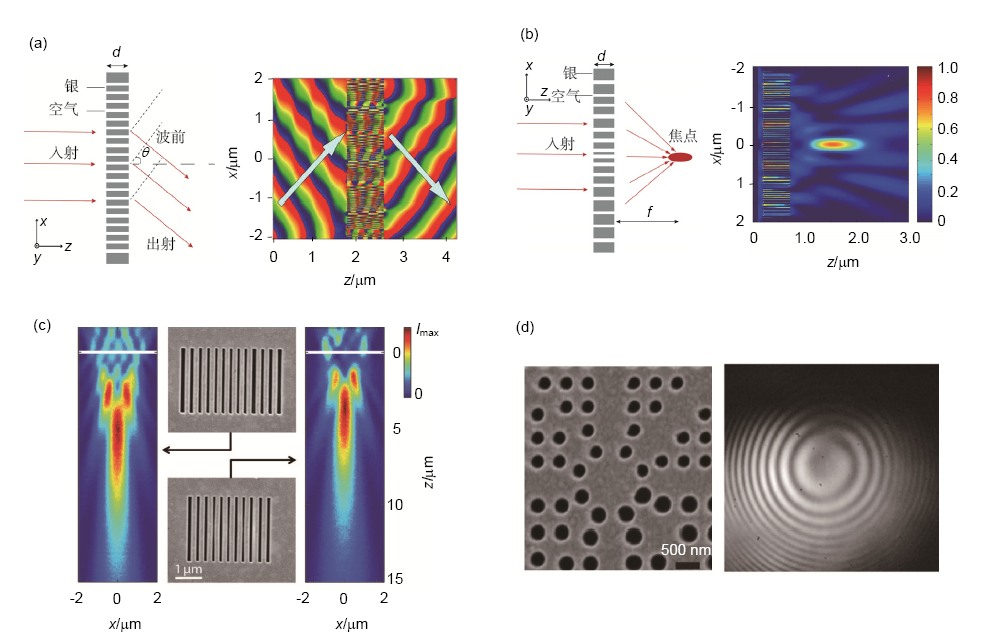
\includegraphics[width=\textwidth]{metasurfaceintro.png}
  \caption{超表面的结构示意图}  \cite{intro01}
  \label{fig:c1fig1}
\end{figure}

尽管超表面目前的具有喜人的应用前景,但是文献调研结果表明,目前的超表面存在一个明显的问题,即超表面一旦被制作出来,它的光学性质就是固定的。这样,对于不同的光学需求而言就需要根据具体问题进行不同的超表面的制备。为此,寻求一种能够在不改变超表面光学器件结构的情况下而能够根据需要改变其光学特性的方法具有重要的实用价值。

\begin{figure}[H] % use float package if you want it here
  \centering
  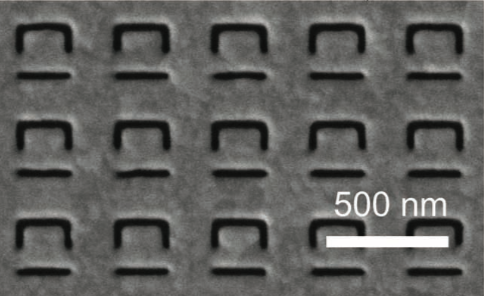
\includegraphics{planestr.png}
  \caption{超表面的周期化二维结构}
  \label{fig:c1fig1}
\end{figure}


\section{GST简介}
\label{sec:first}

GST材料作为一种相变材料,目前已经被广泛应用在光学存储设备中,诸如DVD, CD-ROM中 \cite{savemedia} \cite{tbt}。有关GST材料在存储材料应用场合的挖掘是目前的研究热点之一。GST材料在不同条件下可以实现晶态结构和非晶态结构之间的转化。目前常见的变换晶相结构的方式有两种:热退火和电脉冲,而激光控制GST相变 \cite{laser} 的原理同热退火一致。其中,Ge$_{2}$Sb$_{2}$Te$_{5}$材料在$300 ^{\circ}$C左右退火可以实现从非晶态到晶态到转化,而从$600^{\circ}$C快速退火时可以从晶态转化为非晶态 \cite{GSTbase} 。图 ~\ref{fig:annealing} 展示了退火导致相变的简要过程。

\begin{figure}[H] % use float package if you want it her e
  \centering
  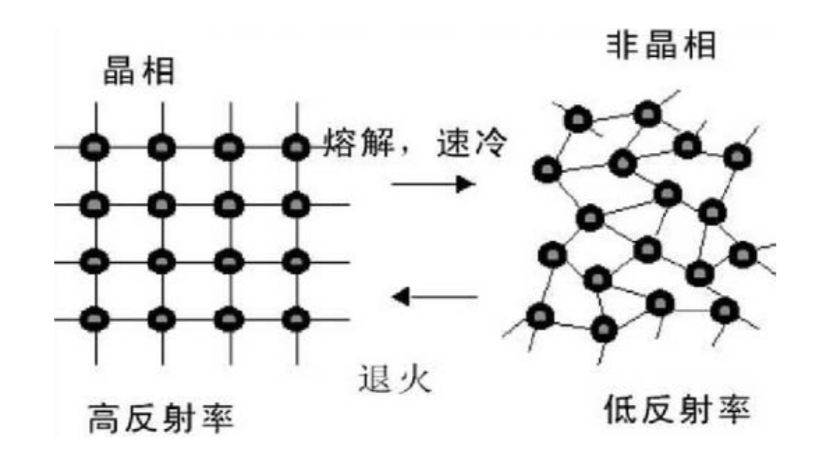
\includegraphics{annealing.png}
  \caption{退火导致相变的简要过程} \cite{GSTbase2}
  \label{fig:annealing}
\end{figure}

同时,GST材料的相变过程也可以通过施加电脉冲来实现。文献 \cite{elePhaseChange} 指出,对于$Ge_{2}Sb_{2}Te_{5}$而言,施加一个短而电压稍高的脉冲(文献中给出的是$\left (6V - 100\ ns \right )$)可以使得GST材料实现从晶态到非晶态的转变;而对于与之相反的过程,文献中给出的电压脉冲形式是$\left (4V - 500\ ns \right )$。如图 ~\ref{fig:elephaseChange} 所示,GST的电特性在相变数十万次之后才会发生显著改变。
\begin{figure}[H] % use float package if you want it here
  \centering
  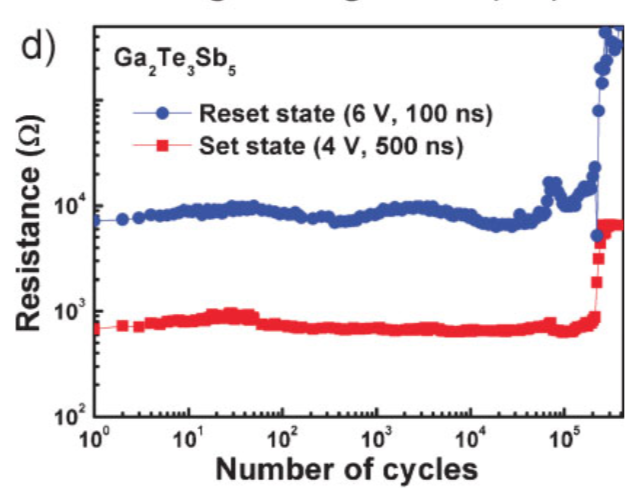
\includegraphics[width = 0.6\textwidth]{elePhaseChange.png}
  \caption{GST材料经过电控的相变过程后电阻的变化} \cite{elePhaseChange2}
  \label{fig:elephaseChange}
\end{figure}

GST本身相变的时间很短,只有纳秒量级 \cite{fast}。如果采用热退火的话,升温和冷却的过程会将这个很短的相变时间淹没,从而难以体现迅速相变的优势;而由于电脉冲诱导GST相变仅需数百纳秒,这可以实现存在相变需求时的快速调节。同时,由于实现纳米尺度的隔热相对困难,而类似尺寸的电极较为易于实现;因此电脉冲控制会更容易实现对GST结晶状态的精确控制。为了实现对各个位置的纳米柱都能进行电位控制,同时又不影响材料的光学特性;我们决定采取ITO-GST-ITO的三层结构,其中ITO为一种透光率高于90\% 的导电材料,是现在应用面比较广的透明电极材料。下图为为了实现对每个纳米柱的控制,我们可以采取的电极排布与加工方法:
\begin{figure}[H] % use float package if you want it here
  \centering
  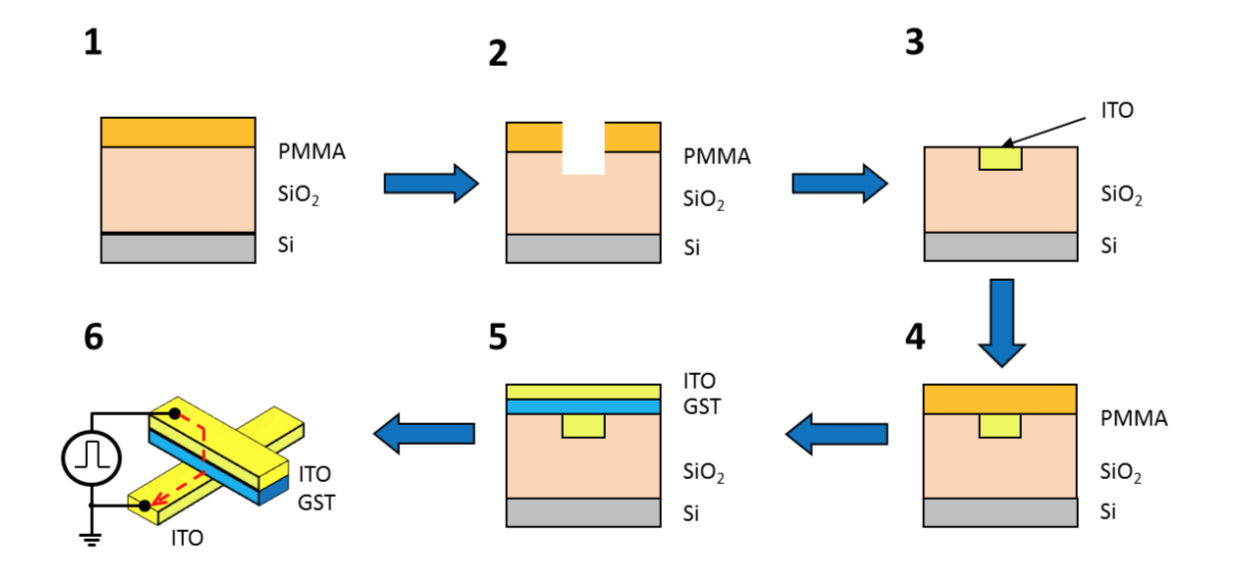
\includegraphics[width = 0.8\textwidth]{itogstito.png}
  \caption{制作三层电极结构的主要过程。}
  \label{fig:elephaseChange1}
\end{figure}

上图展示了制作三层电极结构对主要流程。1. PMMA溅射到了SiO$_{2}$衬底上,并形成一维结构。2. 在氩气氛围下刻出沟槽。3. 在沟槽中以ITO填充,并洗掉表面的PMMA。 4. 生长一层新的PMMA。 5. 按照PMMA形成的一维结构依次溅射GST和ITO。 6. 将三层结构抬离SiO$_{2}$,形成条状电极结构。

Ge$_{2}$Sb$_{2}$Te$_{5}$材料在相变前后折射率的显著差异可以用于制备光学特性可变的超表面光学器件\cite{refocus}。简而言之就是使用GST材料制备超表面中的纳米柱,并通过改变不同位置的纳米柱晶化状态来改变超表面的光学特性。根据文献调研 \cite{GSTnk} 和后续采用椭圆偏振仪测得的结果来看,GST在非晶态时的折射率约为$\left (4 + 0.5i \right )$,而晶化之后的折射率约为$\left (6 + 3i \right )$。作为一种相变材料,GST材料具有相变时间短(150$\ $ns)、相变前后结构确定性好、可循环想变次数多(数十万次)的优点 \cite{GSTbase},因此本论文奖探索利用GST材料来制备可控的超表面的方法。

\begin{figure}[H] % use float package if you want it here
  \centering
  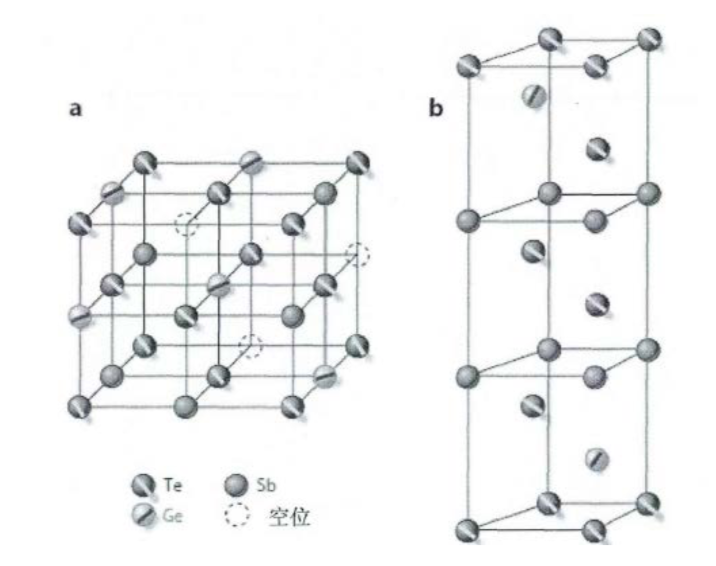
\includegraphics{crystalGST.png}
  \caption{GST材料的两种不同晶化状态} \cite{intro01}
  \label{fig:cGST}
\end{figure}

但是,由于GST材料在晶化与非晶化之间的中间状态尚不明确 \cite{nature},因此本论文将这种材料视为一种具有两种光学特性的材料。为了制作可调超表面光学器件,有两种方式可以考量:
  \begin{itemize}
    \item[-] 强度控制方法:能够有效控制不同位置的、足够大的光强变化;
    \item[-] 相位控制方法: 能够让单个结构单元实现$\left (0, 2\pi \right )$内的相位调节。
  \end{itemize}
目前,对强度调节研究比较好的成果是在1.55 $\mu$m处实现了30 dB的强度隔离\cite{isolation},但这篇文献中实现的是对平面整体的调控而不能实现对平面上各个点的调节。同时,相位控制方法相比于强度控制方法而言,单元尺寸更小,结构可扩展性更好。基于上述原因,我们将后续仿真工作集中在了相位调节上。

\section{实验方法简要说明}
\label{sec:third}
\subsection{GST制备方法}
为了研究GST的相变过程以及光学特性,本论文采用磁控溅射的方法来制备纳米厚度的GST薄膜。磁控溅射指的是在高真空的环境中通入惰性气体,并令惰性气体的离子轰击靶材,使得靶材原子带电并逃逸到空间中,而后在电场作用下 附着到样品上从而实现镀膜的过程\cite{sputtering}。 磁控溅射镀膜的方式具有溅射速率稳定、膜组分稳定性好、重复实验过程之间溅射效果一致性好等特点。图 ~\ref{fig:sputtering} 是磁控溅射的简要原理示意图。
\begin{figure}[H] % use float package if you want it here
  \centering
  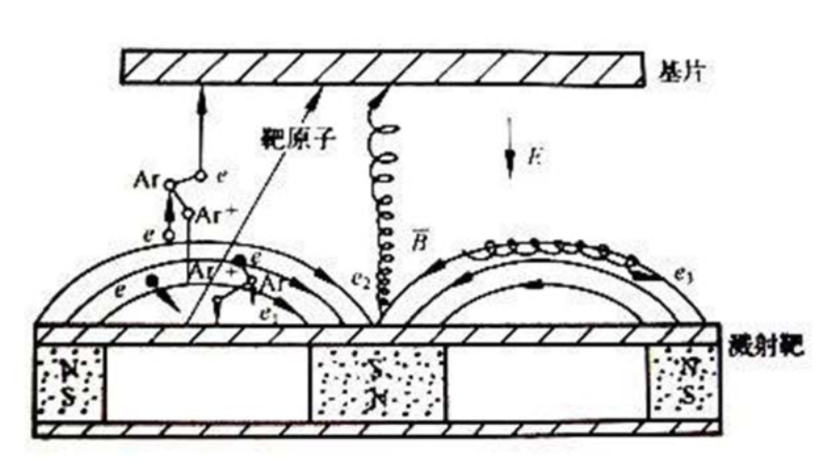
\includegraphics{sputtering.png}
  \caption{磁控溅射原理示意图}\cite{sputtering}
  \label{fig:sputtering}
\end{figure}

与溅射镀膜的质量有关的因素很多,比如溅射的方式、氩气氛围的气压、溅射功率、时间,以及溅射过程中样品是否加热等,而GST材料目前的相关文献非常贫瘠,因此本论文将探索适宜GST的溅射条件。由于GST材料本身的电阻率较高$\left ( >1 k \Omega \cdot{} m \right )$ \cite{ohmofGST},而直流溅射仅适用于导体靶材的溅射。出于对靶材和电极保护的考量,实验过程中仅考虑射频溅射。

\subsection{GST相变方法研究}
本论文用快速退火(RTA)来实现对GST材料的晶化状态的改变。快速退火在氮气氛围下进行,其的目的是防止样片在接近$600\ ^{\circ}$C的温度下受到氧化。根据文献\cite{annealing}调研结果,对于GST材料,无论是晶化过程还是非晶化过程,所需要的退火温度均不超过$500\ ^{\circ}$C。为了防止实验过程中不可避免的样片接触空气对样片造成氧化,我们在退火之前会通5$\ $min $N_{2}$,退火之后会等到反应处冷却至$60\ ^ \circ{} C$以下再取样。但是这并不能彻底杜绝氧化的可能,这点会在后文中展开说明。

\subsection{GST复折射率研究}
本论文使用椭偏仪来对GST的复折射率和厚度进行测量。由于椭偏仪仿真时间过长,因此在本次研究中采用台阶仪来获得样品厚度的数据。(有关其原理详见第 ~\ref{subsection:stage} 小节)
椭圆偏振仪的光路示意图如图 ~\ref{fig:oval} 所示:
\begin{figure}[H] % use float package if you want it here
  \centering
  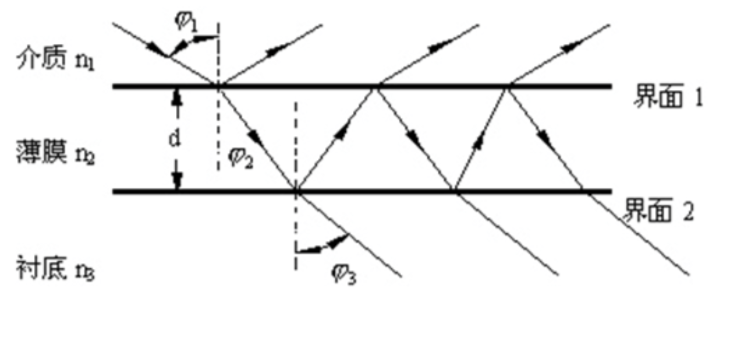
\includegraphics{oval.png}
  \caption{椭圆偏振仪光路示意图}
  \label{fig:oval}
\end{figure}
出射光的波矢与入射波矢之间满足如下方程:
\begin{equation}
G = \frac{E_{rp}}{E_{rs}} \cdot{} \frac{E_{ip}}{E_{is}} = \tan{\Psi \cdot{} e^{i \Delta}} = \frac{r_{1p}+r_{2p}e^{-2i \phi}}{1 + r_{1p}r_{2p}e^{-2i \delta}} \cdot{} \frac{r_{1s}+r_{2s}e^{-2i \phi}}{1 + r_{1s}r_{2s}e^{-2i \delta}}
\end{equation}
其中,$\delta$表示的是膜厚导致的相位差,并满足$\delta = 2 \pi dn_{2} \cos{\phi_{2}} / \lambda$. 椭偏仪通过测量$E_{ip}, E_{is}, E_{rp}, E_{rs}$来拟合薄膜的复折射率和薄膜厚度\footnote{薄膜厚度主要参考台阶仪的测量结果}。
实际上在测量拟合材料的复折射率和厚度中,由于拟合的参数较多,因此容易收敛到一个极值,而这个极值所表征的$\tan{\Psi \cdot{} e^{i \Delta}}$与测量值不符。这种时候需要重新调整拟合中各个参数的初值比较繁琐,因此尽量采用其它途径测量得到与薄膜的复折射率不直接相关的各个参数。

\subsection{GST薄膜光谱透射率和反射率研究}
本论文采用傅立叶光谱仪对GST薄膜对不同波长的光的透过率和反射率进行研究。
傅立叶光谱仪的光学核心是迈克尔逊干涉仪,基本原理是一束光经过分束器之后在待测样品片表面发生干涉,通过测量干涉得到的光强来计算出样品本身的透射率或者反射率,如图 ~\ref{fig:fourier} 所示。
\begin{figure}[H] % use float package if you want it here
  \centering
  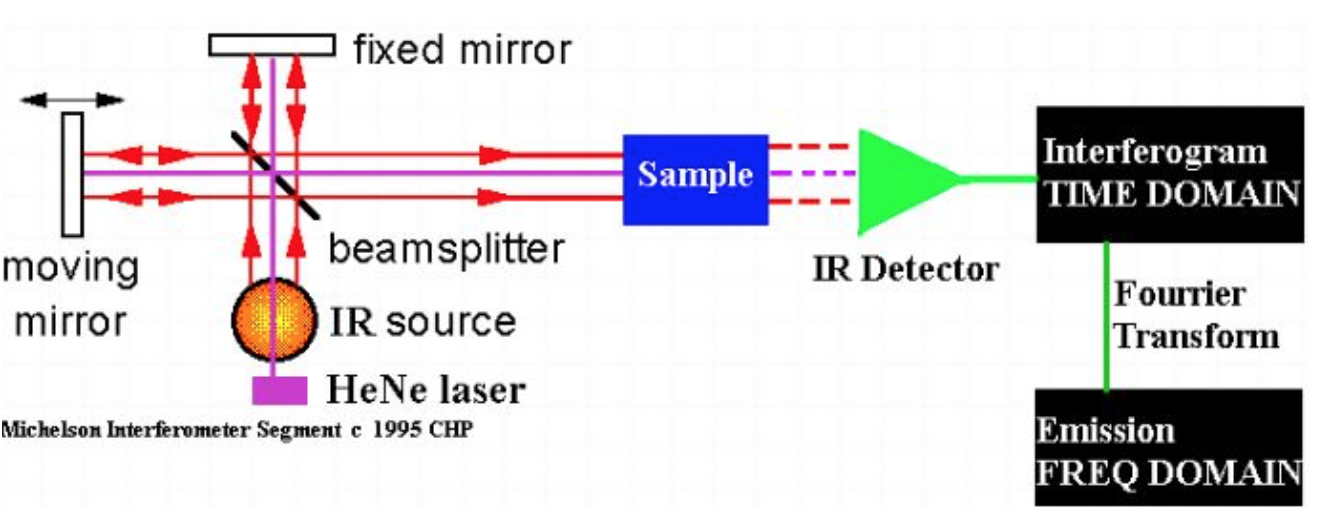
\includegraphics[width=0.8\textwidth]{fourier.png}
  \caption{傅立叶光谱仪原理图}
  \label{fig:fourier}
\end{figure}
和传统的光谱仪相比,傅立叶光谱仪测量的是时域的光强,然后进行傅立叶变换得到频域上的信息,因此具有测量速度快、波数分辨率高的优点。在本项目中,我们为了调查GST材料的光学特性,将这种材料溅射到了铝衬底或者玻璃衬底上,分别得到其反射与透射特性。进而,我们能够从反射特性和透射特性反演出材料的复折射率,与用椭偏仪测定的数据进行对比,从而判断试验结果产生的误差主要来源。

\section{本文结构安排}
本文围绕GST的光学特性进行展开,具体包括优化的超表面的结构,对GST磁控溅射条件的优化,以及对GST薄膜的光学特性研究和结构组分研究。

本论文按照以下方式进行展开:本章主要介绍课题的研究背景,包括超表面的研究现状、GST材料的特性以及实验方法。

第二章介绍了基于FDTD的仿真结果,与优化的超表面结构。

第三章介绍了GST薄膜的制备和光学特性、组分特性的研究。

第四章对本次项目进行总结,并提出了后续的研究思路。
\chapter{基于FDTD的理论仿真}
\label{cha:simulation}

\section{基于GST的可变超表面光学器件结构研究}
\label{sec:second}

我们决定在如图 ~\ref{fig:metaunit}  \cite{GSTnk} 的结构基础上进行优化,这种结构最明显的优点是可扩展性:当在横向增加GST柱子的个数时,GST相变前后导致的折射率变化可以产生更多的可能的调制状态。然而与此同时,结构单元尺寸的增加会导致能够调节的光波长增加,而将三个纳米柱视为一个结构单元是比较折中的一个选择。
\begin{figure}[H] % use float package if you want it here
  \centering
  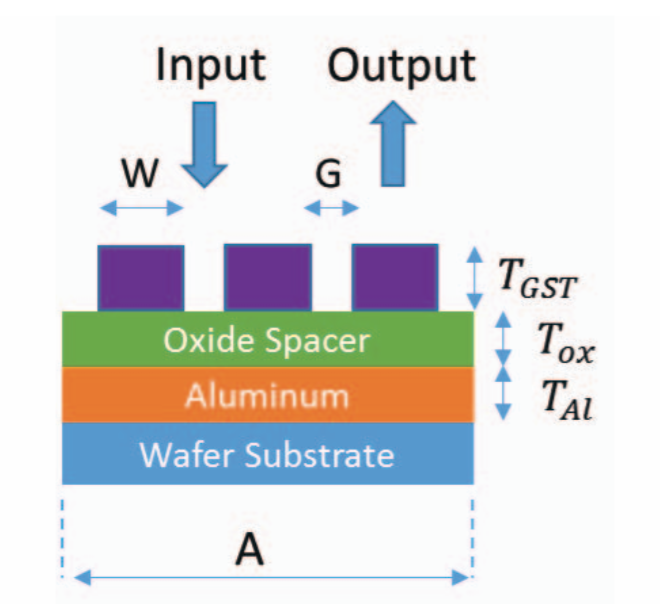
\includegraphics{metaunit.png}
  \caption{可调节纳米柱的结构单元} \cite{GSTnk}
  \label{fig:metaunit}
\end{figure}

在图~\ref{fig:metaunit}所示的结构单元中,每个单元中有三个尺度约为100 nm,间距为47 nm的GST纳米柱。这三个纳米柱排布在50 nm厚的氧化层上,同时加上了铝沉底用来将此结构用作反射器件。根据文献中表明,此结构可以实现在$\left (0,\ 2\pi \right )$范围内的相位调制,但是可调节的相位数目很少。因此,本论文将仿真主要目的集中在增加GST阵列可调节的相位数目。

同时,由于文献 \cite{GSTnk} 中采用的是一维结构,这导致了一个尺度接近$1 \mu m$的结构单元中只有三个纳米柱,而这是一种对空间的浪费。在后续仿真中,我们尝试在一个结构单元中使用$3 \times 3$个GST纳米柱,这样的好处是能够在结构单元尺寸不发生变化的情况下将自由度提升到了原来的平方。

\section{FDTD仿真}
本论文采用FDTD方法对文献所述的功能可调的超表面光学器件单元结构进行仿真与优化。
\subsection{FDTD方法简介}
\label{subsec:fdtd}
FDTD(Finite-Difference Time-Domain),时域有限差分法,核心思想在于把时域麦克斯韦方程转化成差分形式,进而采用数值方法求解。它实现了将计算机不方便处理的旋度方程向差分方程的转化,从而让计算机能够高效地介入电磁场求解的过程中。

以一维麦克斯韦方程为例,在一维场合中,x, y均不影响场量或者介质参数,因此可以表示为
\begin{displaymath}
\frac{\partial E_{x}}{\partial t} = -\frac{1}{\epsilon _{0} \epsilon _{r}} \cdot{} \frac{\partial H_{y}}{\partial z} \qquad \frac{\partial H_{y}}{\partial t} = -\frac{1}{\mu _{0}\mu _{r}} \cdot{} \frac{\partial E_{x}}{\partial z}
\end{displaymath}
使用差分对一阶导数进行近似,我们可以得到
\begin{equation}
\frac{E^{n+1}_{x}(k) - E^{n}_{x}(k)}{\Delta t} = -\frac{1}{\epsilon _0\epsilon _{r}(k)} \cdot{} \frac{H^{n+\frac{1}{2}}_y \left (k+\frac{1}{2} \right) - H^{n+\frac{1}{2}}_y \left (k-\frac{1}{2} \right )}{\Delta z}
\end{equation}
\begin{equation}
\frac{H^{n+\frac{1}{2}}_y \left (k + \frac{1}{2} \right ) - H^{n-\frac{1}{2}}_y \left (k+\frac{1}{2} \right )}{\Delta t} = -\frac{1}{\mu _0\mu _r \left (k+\frac{1}{2} \right )} \cdot{} \frac{E^n_x \left (k+1 \right) - E^n_x \left (k \right )}{\Delta z}
\end{equation}
根据以上两个方程,并使用归一化磁场
\begin{displaymath}
\stackrel{\sim}{H} = \sqrt{\frac{\mu _0}{\epsilon _0}}H
\end{displaymath}

和真空中光速
\begin{displaymath}
c = \frac{1}{\sqrt{\mu _0 \epsilon _0}}
\end{displaymath}

代入,可以得到基于FDTD的迭代公式:

\begin{equation}
\stackrel{\sim}{H}^{n+\frac{1}{2}}_{y} \left (k + \frac{1}{2} \right ) = \stackrel{\sim}{H}^{n - \frac{1}{2}}_y \left (k + \frac{1}{2} \right ) - \frac{c\Delta t}{\mu _r\left (k + \frac{1}{2} \right ) \Delta z} \cdot{} \left ( E^n_x (k + 1) - E^n_x (k) \right )
\end{equation}

\begin{equation}
E^{n + 1}_x \left (k \right ) = E^n_x \left ( k \right ) - \frac {c \Delta t}{\epsilon _r \left (k \right ) \Delta z} \cdot{} \left ( \stackrel{\sim}{H}^{n + \frac{1}{2}}_y \left (k + \frac{1}{2} \right ) - \stackrel{\sim}{H}^{n + \frac{1}{2}}_y \left (k - \frac{1}{2} \right ) \right )
\end{equation}

由于结构参考的文献中采用的是一维结构,而超表面本身蕴含的结构不超过二维;因此对于三维FDTD方程的推导是不必要的。

基于以上原理,我们采用FDTD方法对超表面结构进行仿真。有关仿真的具体过程,在此不加以赘述,只进行一些必要的对结果的讨论。

\subsection{一维情形}
\label{subsec:onedim}
本论文首先实现了对文献所述结构的仿真优化。其中需要的GST材料在可见光-近红外波段的复折射率参数由文献 \cite{GSTnk} 中的曲线粗略得到。有关GST材料在晶态/非晶态的详细折射率如图 ~\ref{fig:nkGST} 所示。
\begin{figure}[H] % use float package if you want it here
  \centering
  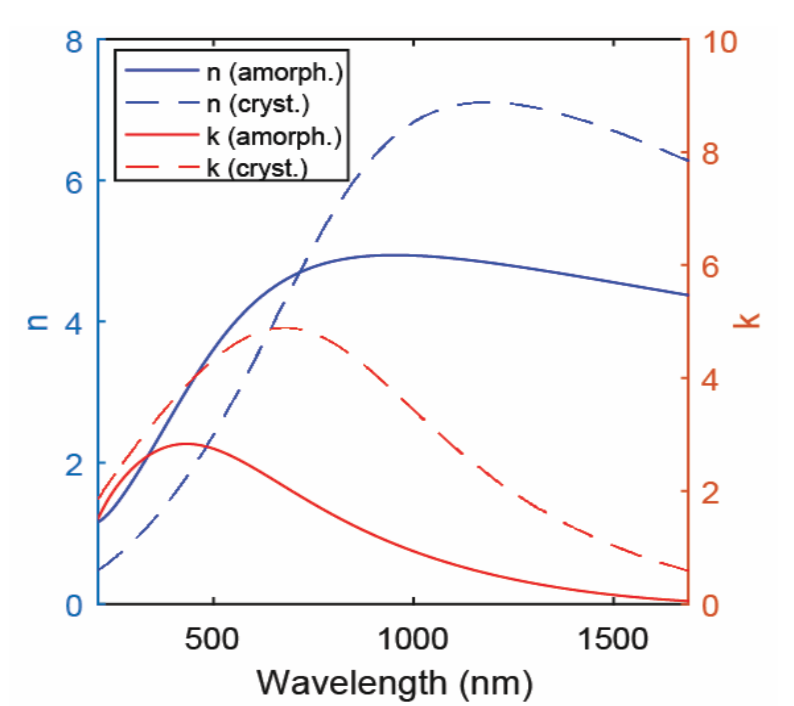
\includegraphics[width=0.5\textwidth]{GSTnk1.png} \cite{GSTnk}
  \caption{GST材料在可见光以及附近的折射率和消光系数}
  \label{fig:nkGST}
\end{figure}

本论文首先进行了对文献中所示结构的验证。一维情况下的结构如图 ~\ref{fig:dstructure} 所示:
\begin{figure}[H] % use float package if you want it here
  \centering
  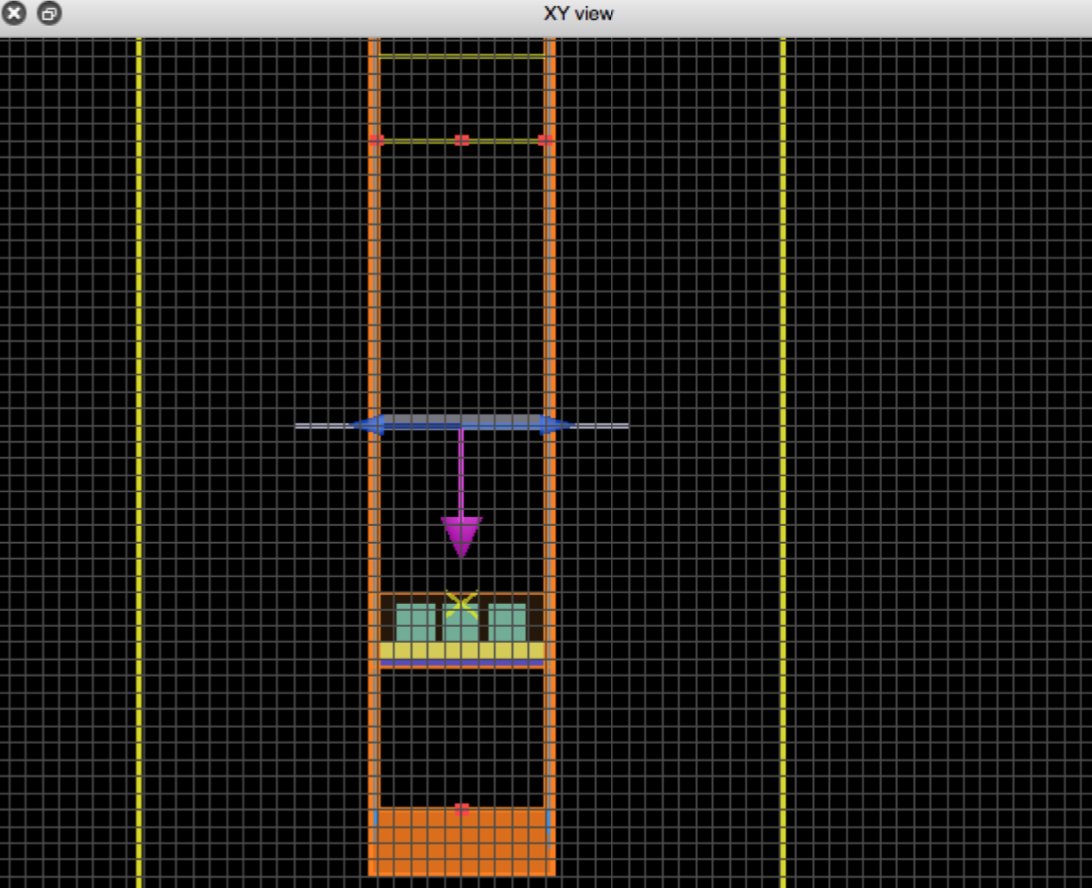
\includegraphics[width = 0.6\textwidth]{1dstructure.png}
  \caption{一维纳米柱结构示意图}
  \label{fig:dstructure}
\end{figure}

其中,三个矩形表示了GST形成的纳米柱。通过预先调入非晶化和晶化状态下的GST材料的$\left (n,k \right )$,我们可以通过设定与更改这三个矩形的材料属性来模拟晶化和非晶化的过程。如果我们用a表示非晶态的GST,而用c来表示晶态的GST材料,那么考虑到对称性,这三个纳米柱组成的结构单元共有$\left (aaa \quad aac \quad acc \quad aca \quad ccc \quad cac \right )$六种状态。由于我们期待着的是一个具有可重复性的结构单元,因此我们将边界条件设置为周期性边界条件来进行仿真。
我们可以得到以下相位曲线:
\begin{figure}[H] % use float package if you want it here
  \centering
  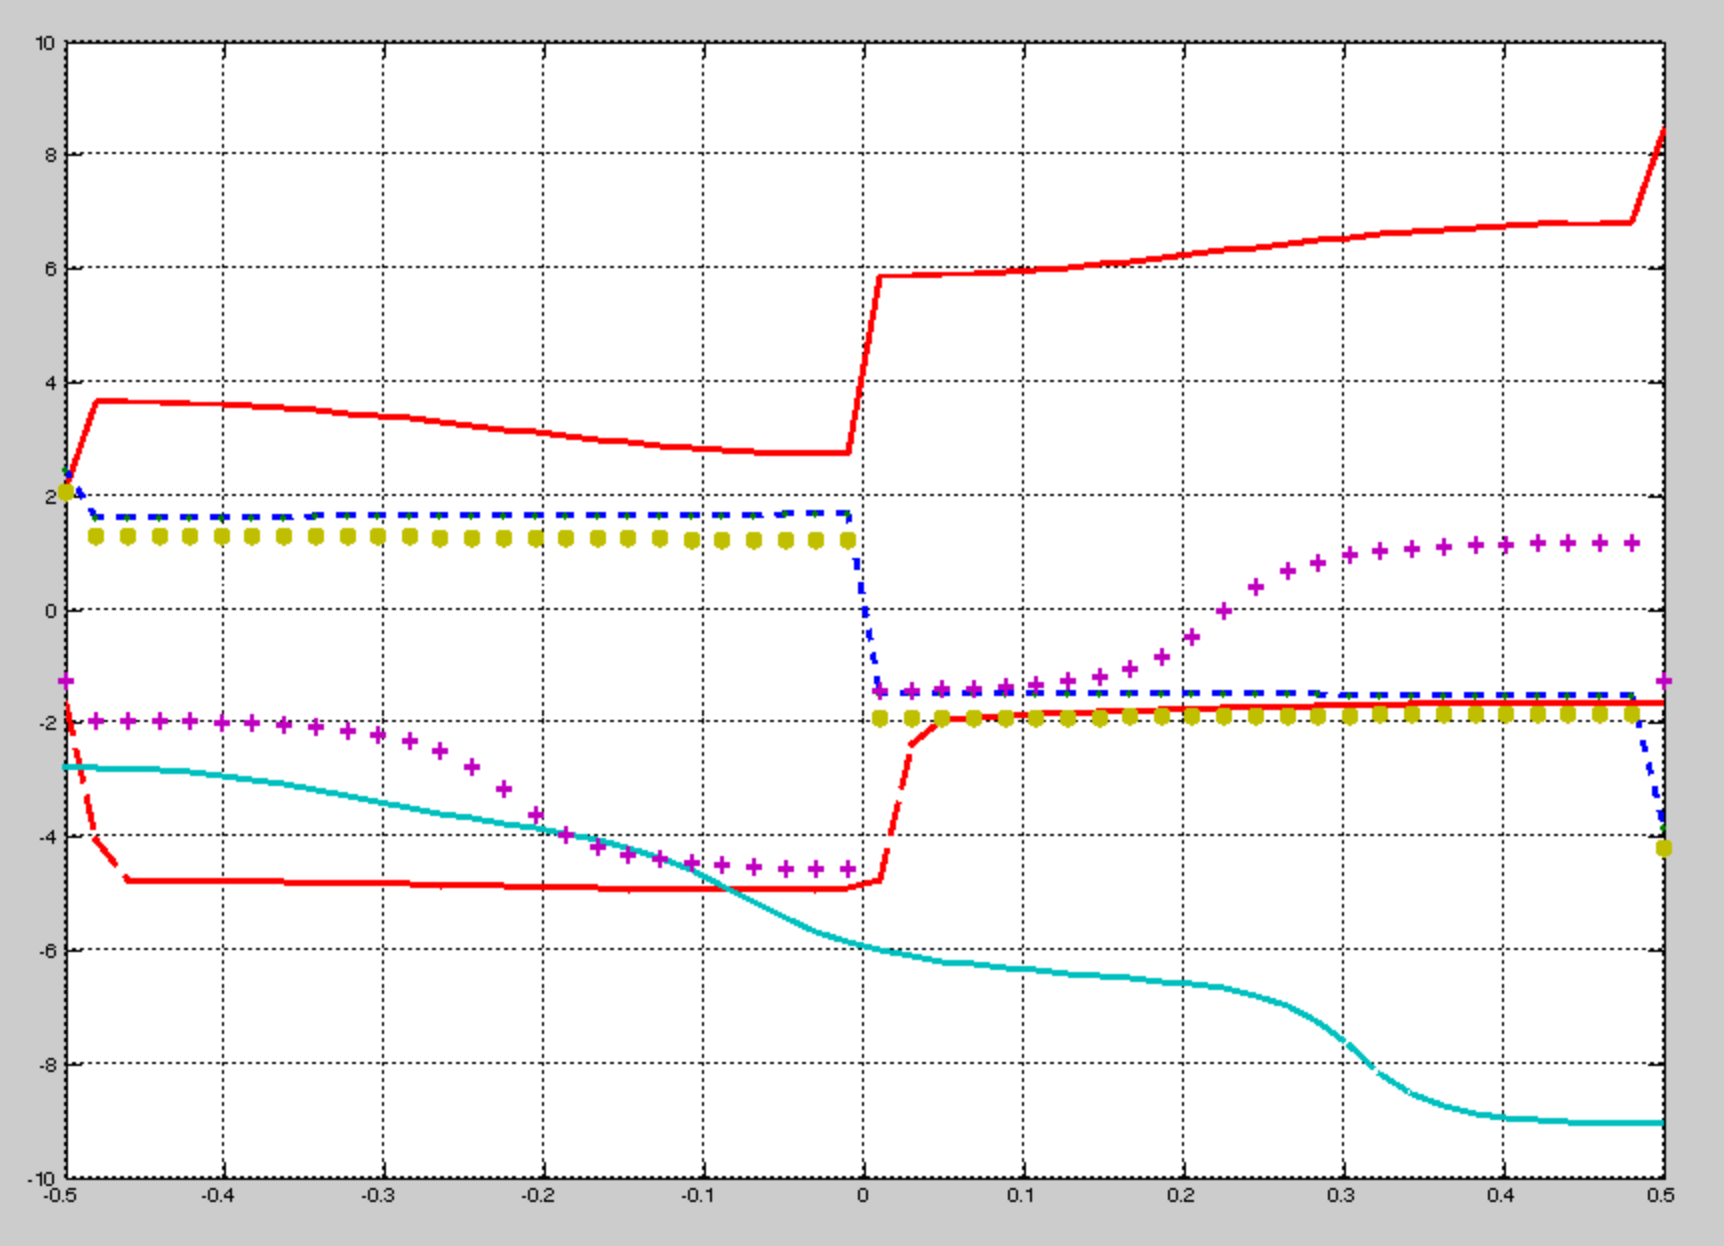
\includegraphics[width = 0.5\textwidth]{1dphase.png}
  \caption{对一维GST纳米柱组合形成的相位分布示意图}
  \label{fig:1dphase}
\end{figure}
零点处的相位随着GST材料晶化状态的仿真结果与文献所述 \cite{metaGST} 十分接近,说明本论文所述的仿真过程和结果是可靠的。但是,在一维情形下,零点附近的相位变化十分剧烈,而零点的相位变化又是我们希望严格受控的,因此在零点附近如此剧烈的相位变化应当在我们后续的结构设计中得到控制。

\subsection{二维情形}
\label{subsec:twodim}
对二维情形的仿真所用到的GST材料的复折射率,同样是基于参考文献 \cite{GSTnk} 中的曲线得到。

二维结构下的结构如图 ~\ref{fig:twodim} 所示,在一维的基础上增加了y方向的结构;除此之外,将纳米柱的形态确定为全等的圆柱体。如下图所示,此超表面的结构单元尺寸约为$1\ \mu m$,仿真所用的光源和检查的平面与反射衬底的底面距离分别为500 nm, 510 nm。
\begin{figure}[H] % use float package if you want it here
  \centering
  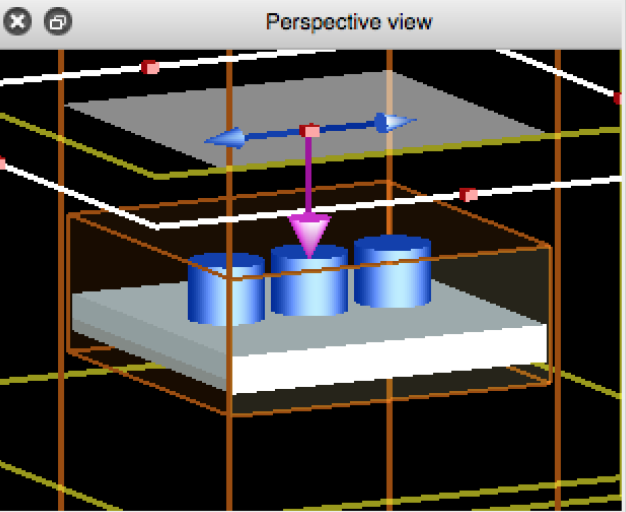
\includegraphics[width = 0.5\textwidth]{twodstructure.png}
  \caption{二维纳米柱结构示意图}
  \label{fig:twodim}
\end{figure}

由于在同一个结构单元内,每个GST纳米柱有晶化和非晶化两种状态,因此在不考虑对称性的情况下一个单独的二维结构单元能够实现$2^9=512$种不同的相位调控。即便考虑对称性,也有86种不用的调节情况(此处的计算用到了P\'olya计数法),远远多于一维情形的六种。为了实现超表面所需的相位调节能力,我们所诉求的是找到尽可能充满$\left (0,\ 2\pi \right )$区间点若干个点。换言之,我们设通过各个GST纳米柱的晶化状态调节能够实现的相位变化集合为A,那么对于任意的$x \in \left (0,\ 2\pi \right )$,均$\exists a \in \mathrm{A}\textrm{和}\delta > 0,\ s.t.\ x \in \left (a - \delta,\ a + \delta \right )$,我们的期望是$\delta$尽可能小。根据经验而言,当$\delta < \pi / 8$时,可以认为基本实现了可控的超表面。

由于二维情况下的可能的晶化种类过多,在此就不一一列举,仅用86种不同的GST纳米柱晶化状态中相位差异较大的两种来说明用GST制作的超表面光学器件具有调节能力:
\begin{figure}[h]
\begin{minipage}{0.3\textwidth}
  \centering
  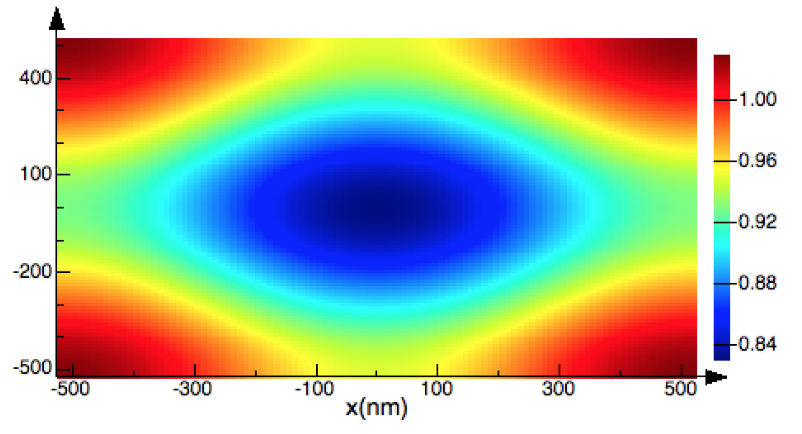
\includegraphics[height = 2.5cm]{tworeflect.png}
  \caption{二维GST纳米柱下的反射强度示意图}
  \label{fig:parallel1}
\end{minipage}\hfill
\begin{minipage}{0.3\textwidth}
  \centering
  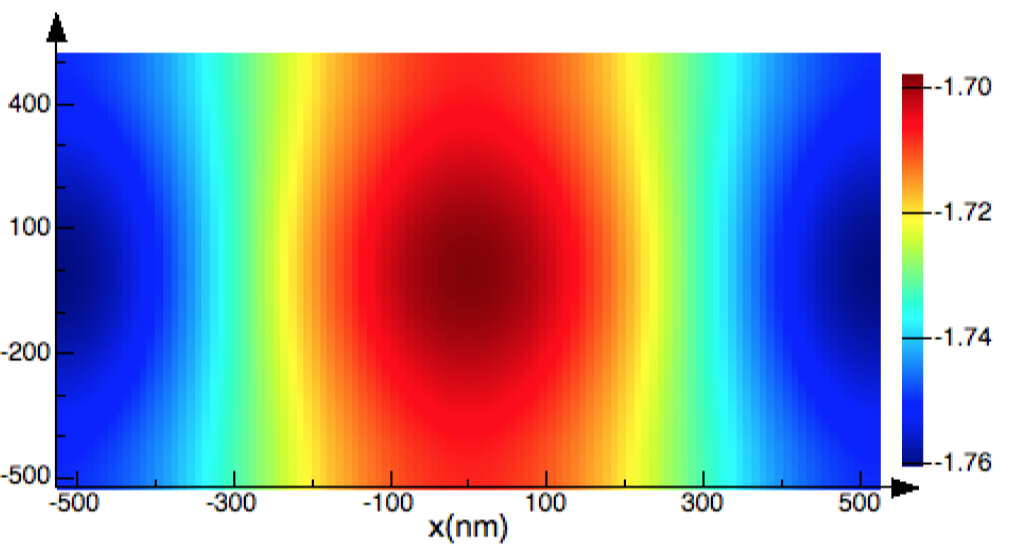
\includegraphics[height = 2.5cm]{twophase1.png}
  \caption{某一个情况下的相位分布}
  \label{fig:parallel2}
\end{minipage}\hfill
\begin{minipage}{0.3\textwidth}
  \centering
  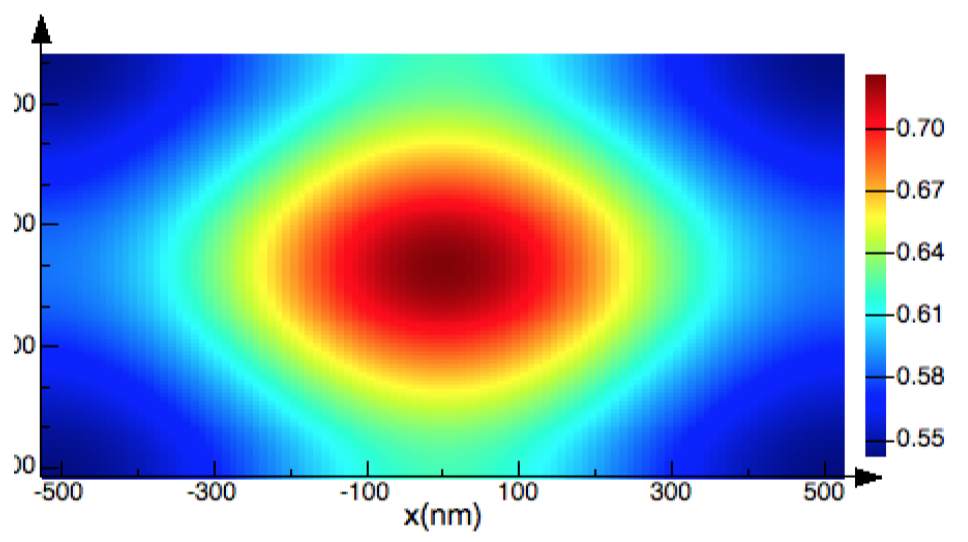
\includegraphics[height = 2.5cm]{twophase2.png}
  \caption{另一个情况下的相位分布}
  \label{fig:parallel2}
\end{minipage}
\end{figure}

从上图中我们可以看出以下几点:
\begin{itemize}
  \item[-] 对于$\lambda \approx 1\ \mu m$的入射光,GST材料的吸收很弱。这说明采用GST制作的超表面光学器件具有损耗小、效率高的特点;
  \item[-] 某个结构单元中各个纳米柱的晶化状态改变前后,在零点处的相位能够有较大的变化;
  \item[-] 无论如何调节某个结构单元中不同纳米柱的晶化状态,零点附近的相位变化是相对平缓的,这是一个明显比一维结构优秀的特点。
\end{itemize}

综上所述,二维结构的调控能力较之一维结构没有本质的提升,但是二维排布的GST纳米柱一维结构所无法比拟的相位稳定性,这使得计算容错性得到提升。

\section{本章小结}
\label{sec:simsumup}
在一维、二维仿真图中,我们可以看到,当把文献所述的GST复折射率采用FDTD仿真时,可以通过GST晶化状态的改变来实现一个能够调控的超表面结构。其中,当GST纳米柱呈一维排布时,零点附近的相位变化跳动比较剧烈;对于二维排布的GST纳米柱,相位平滑程度会好得多。
 \chapter{GST材料的制备方法和特性研究}
\label{chap:03}

\section{采用磁控溅射制备GST薄膜}
\label{sec:exp}

本论文用磁控溅射的方法对纳米厚度的GST薄膜进行制备。本论文准备从溅射气压、溅射功率、溅射时间三个方面优化磁控溅射的条件。为了测量透射结构和反射结构并在这之间进行对比,每组相同的溅射条件下使用铝衬底和玻璃衬底各一进行溅射。其中,溅射气压可用0.2Pa, 0.3Pa, 0.5Pa, 0.6Pa四个参考值;溅射功率可用18W, 36W, 50W, 80W四个参考值;溅射时间可用5min, 10min, 15min, 20min四个参考值。如果采用完全实验,那么总共需要对$4 \times 4 \times 4 = 64$种不同条件下的样品进行溅射;而这其中可能只有若干片是接近符合要求的。为了节约工作量而又不失代表性,我们决定采用正交试验法 \cite{ortho} 来设计实验方案。根据正交试验法,我们需要做16次实验,这些实验的具体条件详见表 ~\ref{tab:ortho} 所示。
\begin{table}[htbp]
  \centering
  \caption{根据正交试验法 \cite{ortho} 确定的实验条件}
  \label{tab:ortho}
  \begin{minipage}[t]{0.8\textwidth} 
    \begin{tabular}{|c|c|c|c|}
    \hline
    序号 & 溅射气压/Pa & 溅射功率/W & 溅射时间/min\\
    \hline \hline
    1 & 0.2 & 18 & 5 \\
    \cline{1-4}
    2 & 0.3 & 18 & 10 \\
    \cline{1-4}
    3 & 0.5 & 18 & 15 \\ 
    \cline{1-4}
    4 & 0.6 & 18 & 20 \\ 
    \cline{1-4}
    5 & 0.2 & 36 & 10 \\ 
    \cline{1-4}
    6 & 0.3 & 36 & 15 \\ 
    \cline{1-4}
    7 & 0.5 & 36 & 20 \\ 
    \cline{1-4}
    8 & 0.6 & 36 & 5 \\
    \cline{1-4}
    9 & 0.2 & 50 & 15 \\
    \cline{1-4}
    10 & 0.3 & 50 & 20 \\
    \cline{1-4}
    11 & 0.5 & 50 & 5 \\
    \cline{1-4}
    12 & 0.6 & 50 & 10 \\
    \cline{1-4}
    13 & 0.2 & 80 & 20 \\
    \cline{1-4}
    14 & 0.3 & 80 & 5 \\
    \cline{1-4}
    15 & 0.5 & 80 & 10 \\
    \cline{1-4}
    16 & 0.6 & 80 & 15 \\
    \hline
    \end{tabular}
  \end{minipage}
\end{table}
根据正交试验法,如果将这三类参数看作三维空间,那么在64种条件下的实验可以看作这个三维空间的正方体以及其内部的各个格点;而正交试验法在这个正方体内对应的点是一些均匀分布的点,因此能够认为这16个点是全部64个点的一个比较有代表性的抽样。同时,对于每组条件溅射两个样片,一片在玻璃衬底上溅射,一片在铝衬底上溅射。溅射得到的部分样片见图 ~\ref{fig:sputtered} 。
\begin{figure}[H] % use float package if you want it here
  \centering
  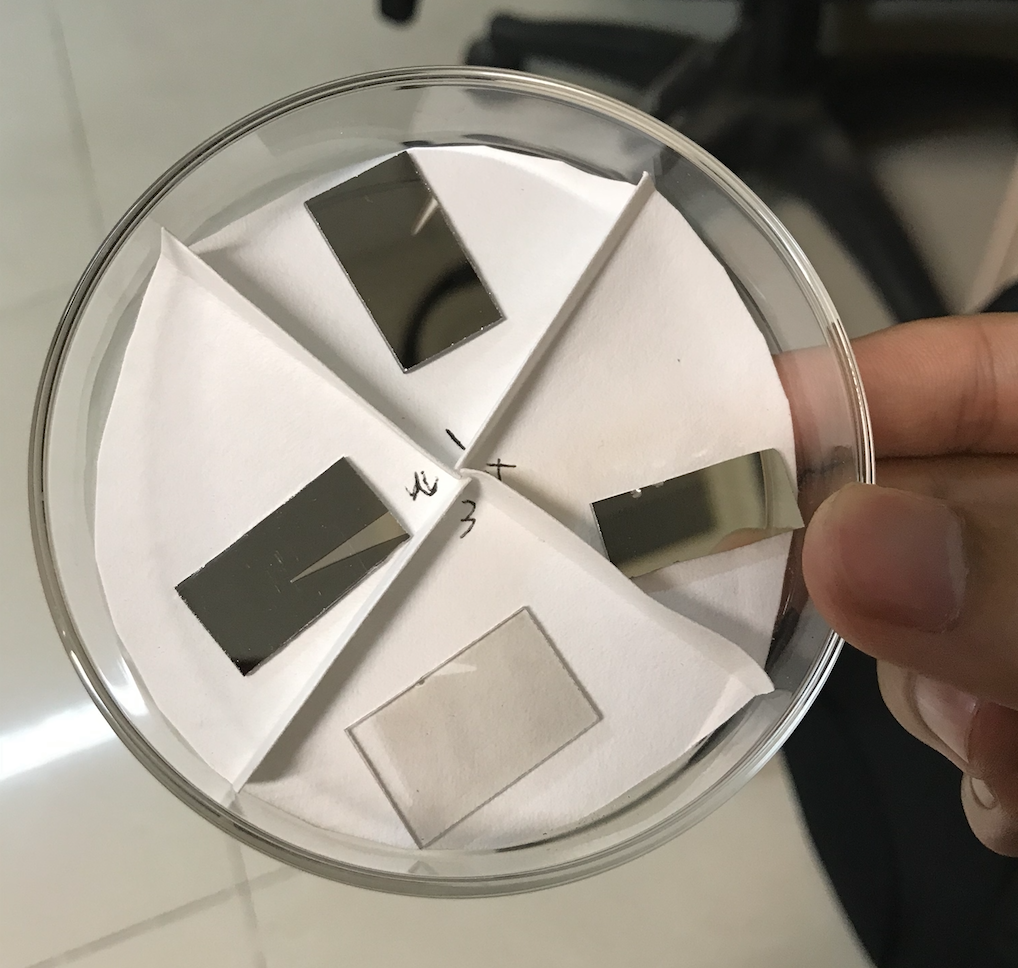
\includegraphics[width=0.5\textwidth]{sputtered.png}
  \caption{溅射得到的部分样片}
  \label{fig:sputtered}
\end{figure}
图 ~\ref{fig:sputtered} 中,一号是0.6 Pa, 36 W, 5 min的条件下在玻璃衬底上溅射的GST薄膜,二号是相同条件下在铝衬底上溅射的GST薄膜;三号是在0.3 Pa, 36 W, 15 min的条件下在玻璃衬底上溅射的GST薄膜,四号是相同条件下在铝衬底上溅射的GST薄膜。

根据得到的样片,我们可以看出在0.2Pa或者0.3Pa的氩气氛围中,溅射功率是18 W或者36 W的话,成膜速度相当慢,不适合用到实际工艺中。而在玻璃表面镀膜的话,当膜厚高于100nm时透明度就会下降到比较低的水准,因此GST材料不适合用作透射结构。根据傅立叶光谱仪的测试结果(详见 ~\ref{sub:testFourier})可以得到,溅射得到的GST薄膜中,材料处于非晶化状态。因此将样品直接做退火流程的时候首先要进行的是从非晶态向晶态转化的退火流程,即在300$\ ^{\circ}$C进行退火。

总体而言,用GST靶材在玻璃/铝衬底上进行磁控溅射均可以得到均一、平整的镀膜。其中经过台阶仪的测量结果,可以得到在0.5Pa, 80W的溅射条件下的成膜速率约为$35nm \cdot{} min^{-1}$并且在显微镜下观察得到的膜表面平整,此条件为本论文所采用。

\section{晶化条件研究}
\label{sec:RTA}
本论文选择热退火的方式来调节其晶化状态。又由于GST相变所需的温度不超过600$\ ^{\circ}$C,而这个温度下GST不易与氮气反应,所以无需采用真空条件下的管式炉进行退火,而采用氮气氛围下的快速退火。

我们得到了32片不同衬底上的GST材料。在每种溅射条件下选择一片进行退火,以便后续进行对比测试。经过300$\ ^{\circ}C$的RTA过程之后,进行了退火的16片样品中,有两片出现了不同程度的损伤。
\begin{figure}[H] % use float package if you want it here
  \centering
  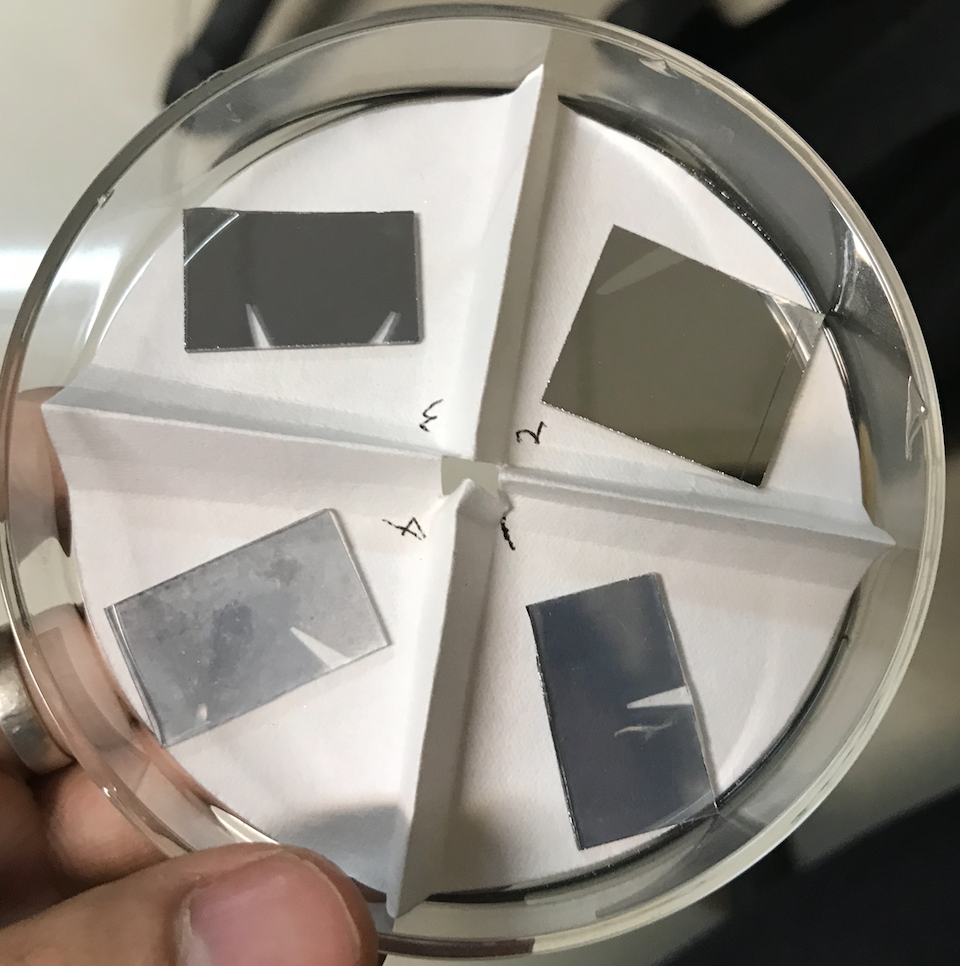
\includegraphics[width=0.5\textwidth]{RTAed.png}
  \caption{部分退火之后的样片形貌}
  \label{fig:RTA}
\end{figure}
由图 ~\ref{fig:RTA} 可以看出,编号为1和四的两片出现了不同程度的表面不平整的现象。由于出现问题的样片集中在直接将GST镀到玻璃上的,因此推断GST不适合直接在玻璃上进行溅射。因此在制备纳米厚度的GST薄膜过程中需要在玻璃上镀一层铝或者钛。

\section{厚度研究}
首先,我们关心的是溅射速度。为此,我们使用台阶仪来对厚度有一个直观的估计。台阶仪的原理之前已经提及过,在此不予赘述。在溅射功率为18W或者36W;同时溅射气压是0.2Pa或者0.3Pa时,即便在20min的溅射条件下也无法用台阶仪测得其准确结果,判断其厚度在100nm以下。实际上由于表面平整度和清洁程度的问题,能够看出明显台阶的只有若干片。其中较为典型的如下图所示:
\begin{figure}[H] % use float package if you want it here
  \centering
  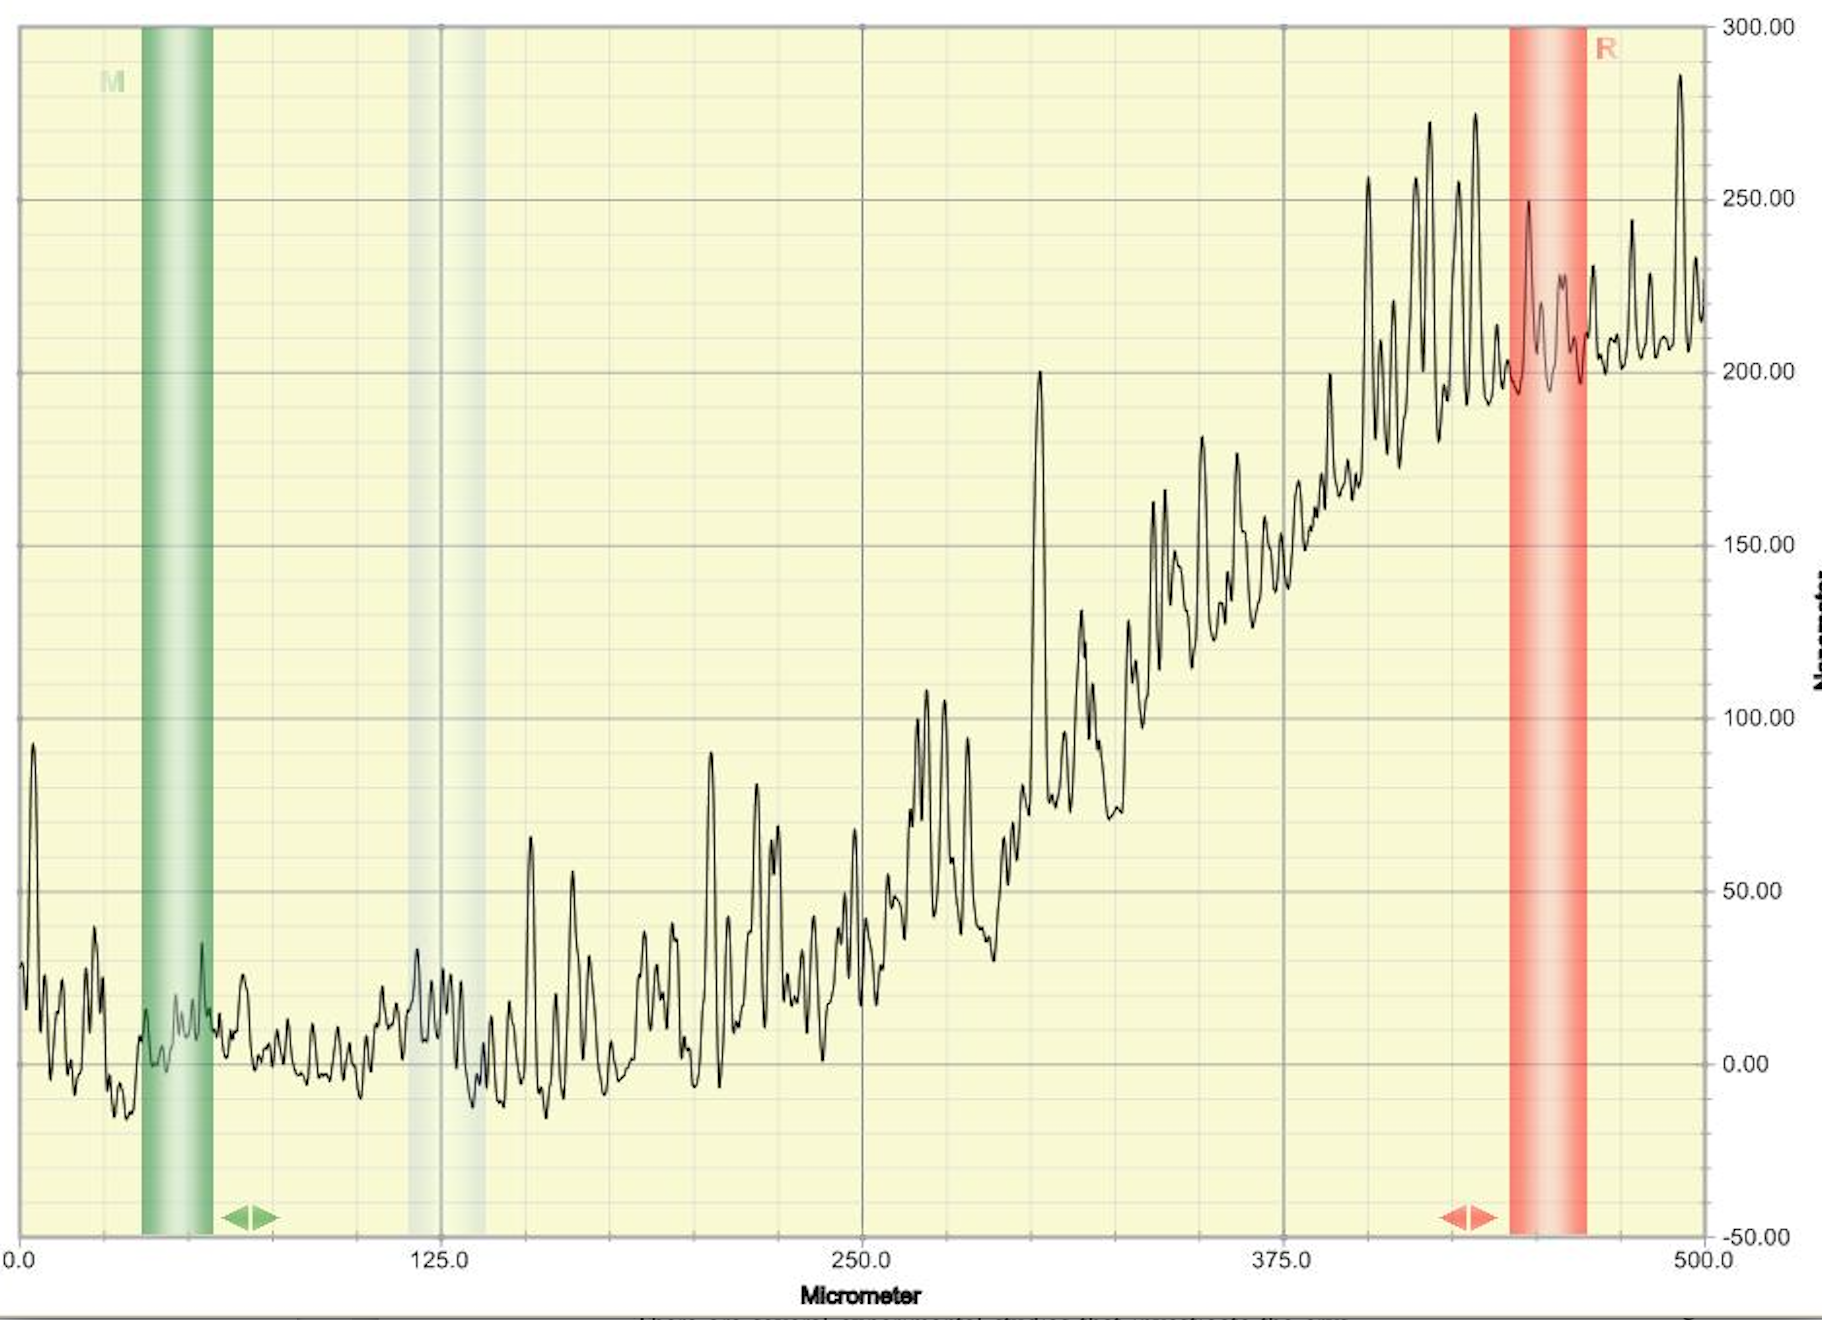
\includegraphics[width=0.5\textwidth]{GSTstep.png}
  \caption{溅射条件:50W,0.5Pa,5min}
  \label{fig:step}
\end{figure}
同时,当把溅射功率提升到80W的时候,溅射速率没有显著变化。由台阶仪的数据可以看出在这种溅射条件下,溅射速率约为$35nm \cdot{} min^{-1}$.

\section{光学特性测试}
\label{sub:testFourier}
本论文准备利用傅立叶光谱仪来测得GST材料的光学特性。其中,对于衬底是玻璃的GST膜,我们更关心它的透射特性;而对于衬底是铝的GST膜,我们更关心它的反射特性。经过测试,我们发现GST的透射特性基本随着波长的增加而增加,对于$\lambda \approx 1.4\ \mu m$以上的入射光基本可以视为透明材料(见图 ~\ref{fig:trans} )。

而对于铝衬底的GST膜,其反射率有明显的峰值,并且随着溅射条件(厚度)不同而不同,推测为光在上下表面发生干涉导致的(见图 ~\ref{fig:reflect})。
\begin{figure}[H] % use float package if you want it here
  \centering
  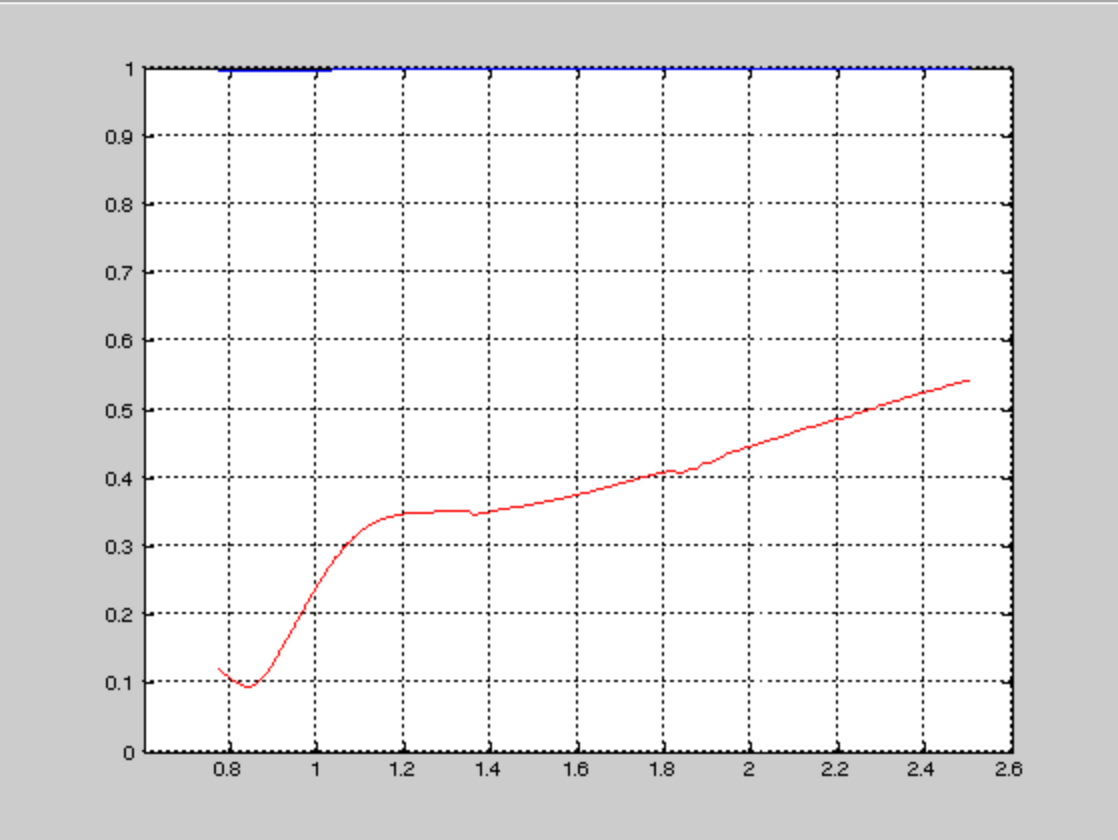
\includegraphics[width=0.8\textwidth]{GSTtrans.png}
  \caption{GST薄膜的透射曲线}
  \label{fig:trans}
\end{figure}
\begin{figure}[H] % use float package if you want it here??
  \centering
  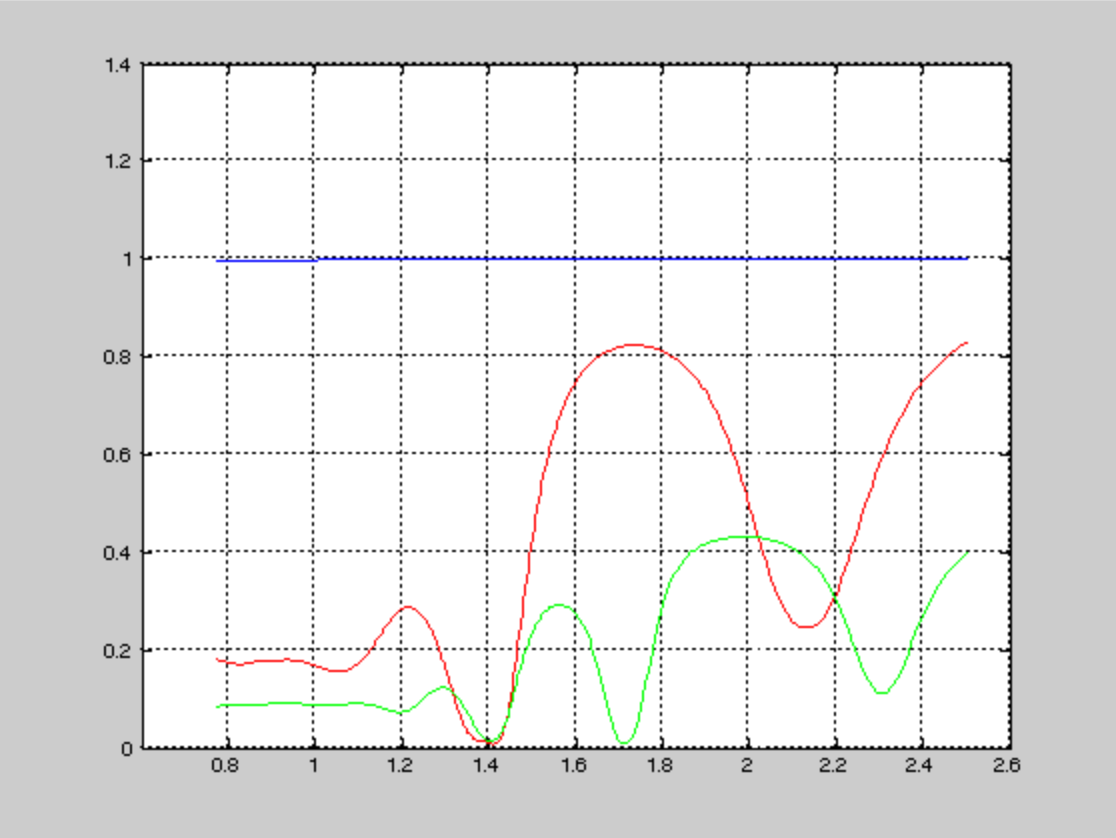
\includegraphics[width=0.8\textwidth]{GSTreflect.png}
  \caption{GST薄膜的反射曲线}
  \label{fig:reflect}
\end{figure}



\subsection{折射率测试}
本论文采用椭圆偏振仪测量GST薄膜的折射率,并以此推断材料的晶化状态,它和后面的XPS是我们判断退火是否有效的重要依据。
对椭偏仪的数据进行拟合的主要理论依据是柯西色散方程:
\begin{equation}
n\left ( \lambda \right ) = \sum_{i=0}^{\infty} \left (\frac{a_{k}}{\lambda ^{2k}} \right )
\end{equation}
在实际拟合过程中,我们只关心这个色散方程的前5项,以及薄膜厚度。拟合得到的曲线和椭偏仪测量的曲线总是存在较大的误差,可能的原因是各个部分的材料组分不稳定,或者材料表面不够平整。实际测得的GST材料的复折射率与最终拟合曲线和实测曲线的误差如下图所示:
\begin{figure}[H] % use float package if you want it here
  \centering
  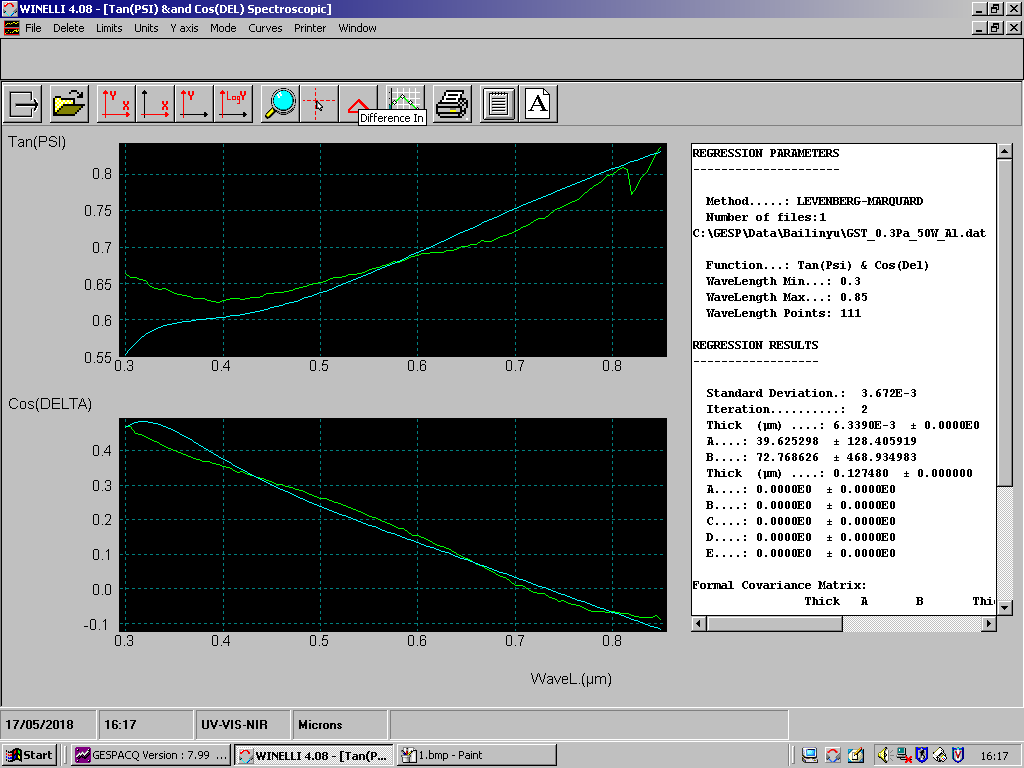
\includegraphics[width=0.8\textwidth]{ovaltest.png}
  \caption{拟合曲线和实测曲线的误差}
  \label{fig:oval}
\end{figure}
\begin{figure}[H] % use float package if you want it here
  \centering
  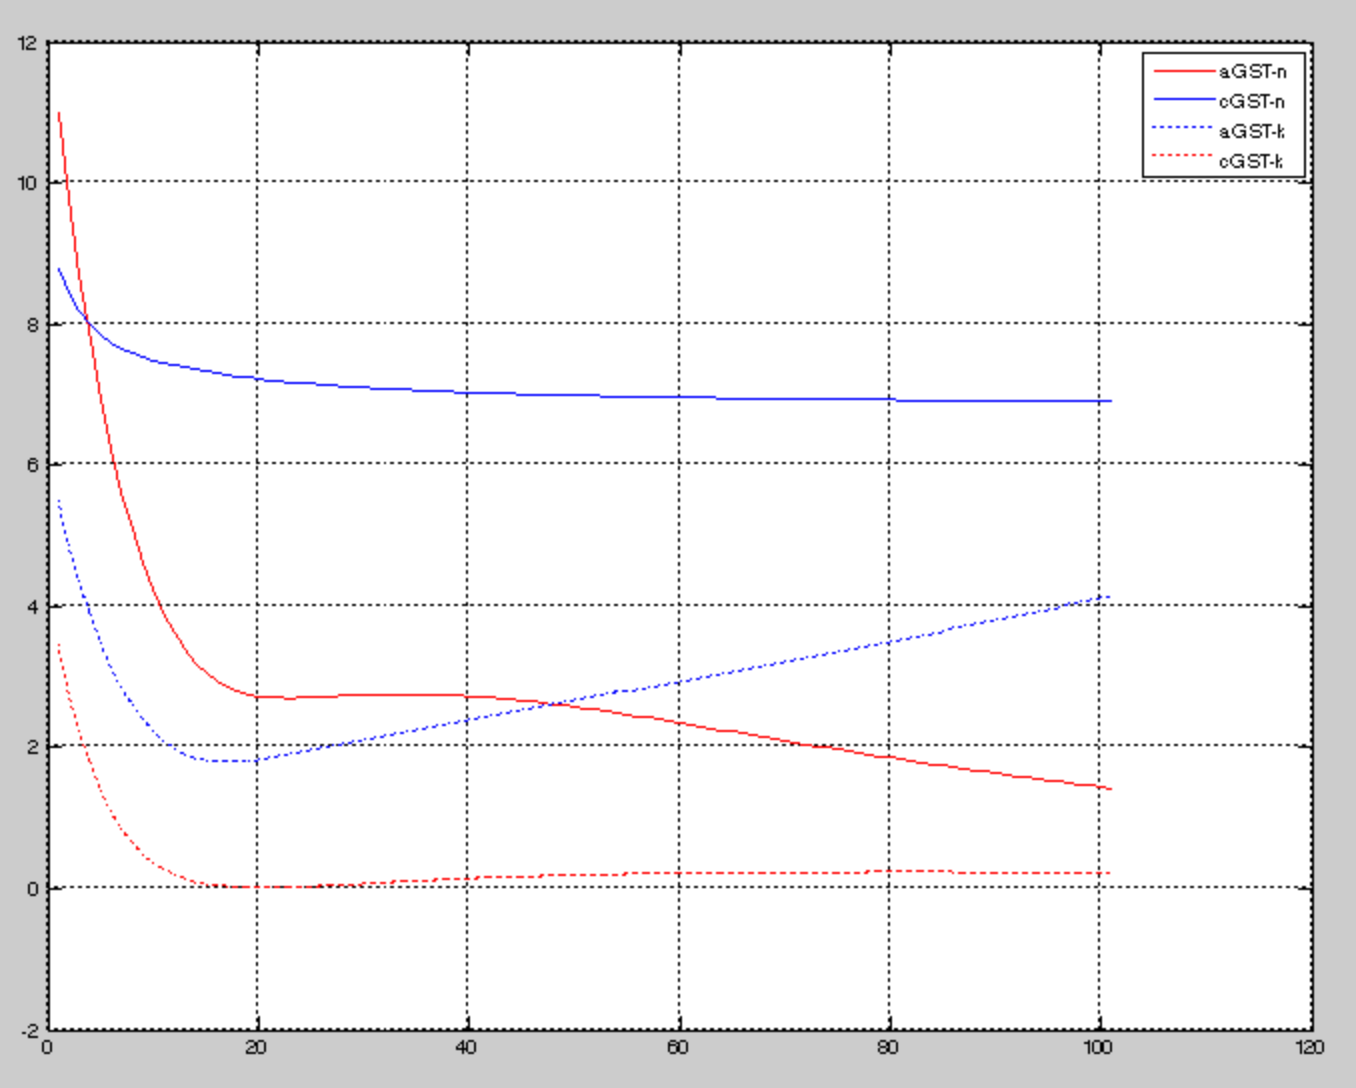
\includegraphics[width=0.8\textwidth]{GSTnktested.png}
  \caption{拟合结果对应的GST复折射率}
  \label{fig:nktested}
\end{figure}
\begin{figure}[H] % use float package if you want it here
  \centering
  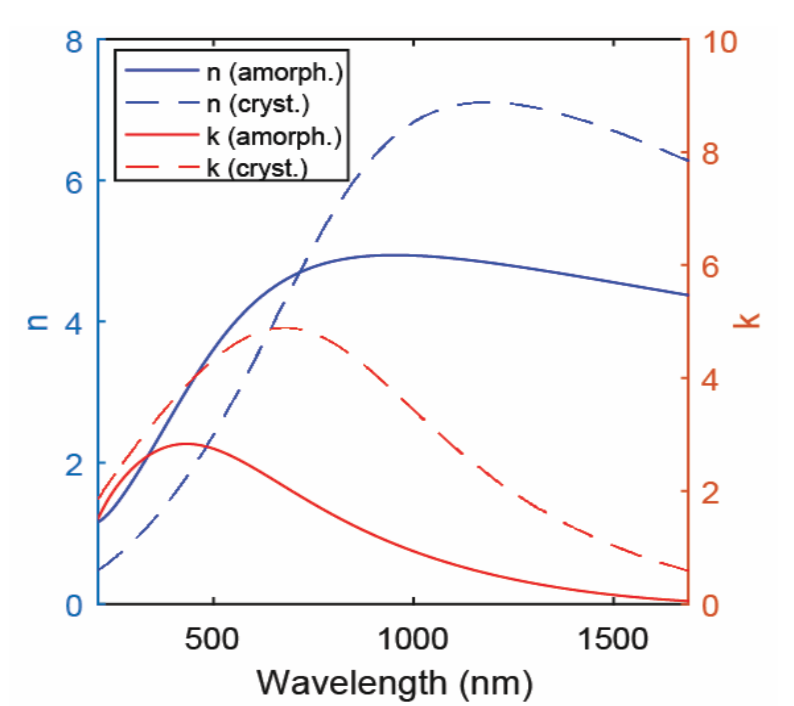
\includegraphics[width=0.5\textwidth]{GSTnk1.png} \cite{GSTnk}
  \caption{文献\cite{GSTnk}中给出的GST复折射率}
  \label{fig:nkGST}
\end{figure}


由以上数据并将上述数据和文献中的数据进行对比,我们可以发现尽管测得的GST复折射率同文献中提及的在数值上表现得较为接近,但是与预想的曲线存在趋势上的差距。在后续研究中,制作更为干净、更为平整的GST薄膜以及提升衬底金属的质量;同时,对柯西色散曲线的拟合可能需要尝试更多的初值,或者考虑尝试更多的色散模型来对椭偏仪测量得到的数据进行更准确的拟合。

\section{GST薄膜表面成分分析}
\label{sub:test_XPS}
本论文采用X射线光子能谱来对溅射得到的GST薄膜表面成分进行分析,以下是分析结果:
\begin{table}[htbp]
\centering
\caption{XPS测试结果}
\label{tab:subtable}
\subcaptionbox{GST未退火时的表面组分}
{
\begin{tabular}{|c|c|}
\toprule[1.5pt]
元素类型与轨道电子 & 含量百分比 \\
\midrule[1pt]
C1s & 28.04 \\
\hline
O1s & 49.02 \\
\hline
Ge2p & 4.75 \\
\hline
Sb3d & 3.61 \\
\hline
Te3d & 14.58 \\
\bottomrule[1.5pt]
\end{tabular}
}
\hskip1cm
\subcaptionbox{退火后的GST表面组分}
{
\begin{tabular}{|c|c|}
\toprule[1.5pt]
元素类型与轨道电子 & 含量百分比 \\
\midrule[1pt]
C1s & 24.8 \\
\hline
O1s & 58.48 \\
\hline
Ge2p & 3.74 \\
\hline
Sb3d & 4.28 \\
\hline
Te3d & 8.71 \\
\bottomrule[1.5pt]
\end{tabular}
}
\end{table}
\\
通过 ~\ref{tab:subtable} 的结果可以得到,无论GST薄膜是否经过退火,表面都有大量的碳、氧杂质。其中,碳的引入是必然的,因为XPS测试通常使用碳原子进行定标;而氧的引入可能是因为从溅射/退火到后来送样期间时间较长,表面氧化严重。同时组分中Ge, Sb, Te的比例大致保持着$2:2:5$的化学计量数之比,这说明GST的各个组分之间在溅射前后相对稳定。同时,表层的氧原子含量过高,这点也可能和椭偏仪的测试结果不尽如人意有关。
\chapter{总结}
\label{chap:04}

本论文主要结论包括:
\begin{enumerate}
	\item 仿真表明二维排布的GST纳米柱阵列形成的超表面光学器件可以实现功能可调的目的。
	\item 采用磁控溅射的方式制备纳米厚度的GST薄膜时,气压不应低于0.3Pa。
	\item GST薄膜在制备过程中可能会被氧化,从而使成膜质量受到影响。
	\item XPS分析结果表明,退火过程会对薄膜表面进行更多的氧元素。
	\item GST材料在可见光-近红外波段更接近一种反射材料,$\lambda > 1.4\ \mu m$时透过率达到80\%。
	\item GST材料在晶态和非晶态中的折射率、色散方程参数确实有显著差异,这个差异使得我们最初设计的超表面结构具有一定调节能力。
\end{enumerate}

尽管本次研究已经得到了一些结论,但是为了实现制作功能可调的超表面的目标,尚需展开更深入的研究,例如:
\begin{enumerate}
	\item 温控GST相变中氧元素的来源及解决方法;
	\item 电控GST实现相变的具体方法和条件,尤其是电控GST材料相变的条件\cite{nature1}和GST材料在晶态和非晶态之间状态的光学特性\cite{middle}。
	\item 基于GST的超表面结构光学器件的制备。
\end{enumerate}

\begin{thebibliography}{99}
\bibitem{intro01} Chu C H, Tseng M L, Chen J, et al. Active dielectric metasurface based on phase‐change medium[J]. Laser \& Photonics Reviews, 2016, 10(6): 986-994.

\bibitem{intro02} Guo Y. Advances of dispersion-engineered metamaterials[J]. 光电工程, 2017 (2017 年 01): 124-125.

\bibitem{elePhaseChange} Kao K F, Lee C M, Chen M J, et al. $\mathrm{Ge_{2}Sb_{2}Te_{5}}$—A Candidate for Fast and Ultralong Retention Phase‐Change Memory[J]. Advanced Materials, 2009, 21(17): 1695-1699.

\bibitem{elePhaseChange2} Au Y Y, Bhaskaran H, Wright C D. Phase-change devices for simultaneous optical-electrical applications[J]. Scientific reports, 2017, 7(1): 9688.

\bibitem{GSTnk} Colburn S, Zhan A, Majumdar A, et al. Active metasurfaces based on phase-change memory material digital metamolecules[J].

\bibitem{speedlimit} Loke D, Lee T H, Wang W J, et al. Breaking the speed limits of phase-change memory[J]. Science, 2012, 336(6088): 1566-1569.

\bibitem{savemedia} Pandian R, Kooi B J, Palasantzas G, et al. Nanoscale Electrolytic Switching in Phase‐Change Chalcogenide Films[J]. Advanced Materials, 2007, 19(24): 4431-4437.

\bibitem{fast} Chen B, de Wal D, ten Brink G H, et al. Resolving crystallization kinetics of GeTe phase-change nanoparticles by ultrafast calorimetry[J]. Crystal Growth \& Design, 2017.

\bibitem{tbt} Liu H, Liu P, Bian L, et al. Electrically tunable terahertz metamaterials based on graphene stacks array[J]. Superlattices and Microstructures, 2017, 112: 470-479.

\bibitem{fourier} Curran P J, Dungan J L. Estimation of signal-to-noise: a new procedure applied to AVIRIS data[J]. IEEE Transactions on Geoscience and Remote sensing, 1989, 27(5): 620-628.

\bibitem{sputtering} 李维娟主编. 材料科学与工程实验指导书[M]. 北京:冶金工业出版社, 2003, 26(5): 352-354.

\bibitem{ortho} 陈磊, 简炜. 计算机实现基于正交试验的测试用例自动生成[J]. 信息安全与技术, 2011, 5: 031.

\bibitem{isolation} Jafari M, Rais-Zadeh M. An ultra-high contrast optical modulator with 30 dB isolation at 1.55 $\mu$m with 25 THz bandwidth[C]//Photonic Fiber and Crystal Devices: Advances in Materials and Innovations in Device Applications XI. International Society for Optics and Photonics, 2017, 10382: 1038211.

\bibitem{laser} Tian X, Li Z Y. An Optically-Triggered Switchable Mid-Infrared Perfect Absorber Based on Phase-Change Material of Vanadium Dioxide[J]. Plasmonics, 2017: 1-10.

\bibitem{ohmofGST} Wuttig M, Yamada N. Phase-change materials for rewriteable data storage[J]. Nature materials, 2007, 6(11): 824.

\bibitem{metaGST} Colburn S, Zhan A, Deshmukh S, et al. Metasurfaces based on nano-patterned phase-change memory materials[C]//Lasers and Electro-Optics (CLEO), 2017 Conference on. IEEE, 2017: 1-2.

\bibitem{structure} Hsiao H H, Chu C H, Tsai D P. Fundamentals and applications of metasurfaces[J]. Small Methods, 2017.

\bibitem{tunable} Xu Y, Tennyson E M, Kim J, et al. Active Control of Photon Recycling for Tunable Optoelectronic Materials[J]. Advanced Optical Materials, 2018, 6(7): 1701323.

\bibitem{refocus} Schultz Carstensen M, Zhu X, Esther Iyore O, et al. Holographic Resonant Laser Printing of metasurfaces using plasmonic template[J]. ACS Photonics, 2018.

\bibitem{GSTbase} Ryu S W, Oh J H, Choi B J, et al. SiO$_{2}$ incorporation effects in Ge$_{2}$Sb$_{2}$Te$_{5}$ films prepared by magnetron sputtering for phase change random access memory devices[J]. Electrochemical and solid-state letters, 2006, 9(8): G259-G261.

\bibitem{nature} Hosseini P, Wright C D, Bhaskaran H. An optoelectronic framework enabled by low-dimensional phase-change films[J]. Nature, 2014, 511(7508): 206.

\bibitem{nature1} Hosseini P, Wright C D, Bhaskaran H. An optoelectronic framework enabled by low-dimensional phase-change films[J]. Nature, 2014, 511(7508): 206.

\bibitem{nature2} Chabinyc M L, Wong W S, Arias A C, et al. Printing methods and materials for large-area electronic devices[J]. Proceedings of the IEEE, 2005, 93(8): 1491-1499.

\bibitem{GSTbase2} Raeis-Hosseini N, Rho J. Metasurfaces based on phase-change material as a reconfigurable platform for multifunctional devices[J]. Materials, 2017, 10(9): 1046.

\bibitem{phasechangememory} Terao M, Morikawa T, Ohta T. Electrical phase-change memory: fundamentals and state of the art[J]. Japanese Journal of Applied Physics, 2009, 48(8R): 080001.

\bibitem{middle} Komar A, Paniagua-Domínguez R, Miroshnichenko A, et al. Dynamic beam switching by liquid crystal tunable dielectric metasurfaces[J]. ACS Photonics, 2018.

\bibitem{vib} Shportko K, Zalden P, Lindenberg A M, et al. Anharmonicity of the vibrational modes of phase-change materials: A far-infrared, terahertz, and Raman study[J]. Vibrational Spectroscopy, 2018, 95: 51-56.

\bibitem{XPS1} Moulder J. Handbook of X-ray photoelectron spectroscopy: a reference book of standard spectra for identification and interpretation of XPS data[M]. Eden Prairie, Minnesota: Physical Electronics Division, Perkin-Elmer Corporation, 1992.

\bibitem{XPS2} Watts J F, Wolstenholme J. An introduction to surface analysis by XPS and AES[J]. 2003.

\end{thebibliography}



%%% 其它部分
\backmatter

%% 本科生要这几个索引,研究生不要。选择性留下。
% 插图索引
\listoffigures
% 表格索引
\listoftables
% 公式索引
\listofequations


%% 参考文献
% 注意:至少需要引用一篇参考文献,否则下面两行可能引起编译错误。
% 如果不需要参考文献,请将下面两行删除或注释掉。
% 数字式引用
\bibliographystyle{thuthesis-numeric}
% 作者-年份式引用
% \bibliographystyle{thuthesis-author-year}
% \bibliography{ref/refs}


%% 致谢
% 如果使用声明扫描页,将可选参数指定为扫描后的 PDF 文件名,例如:
% \begin{acknowledgement}[scan-statement.pdf]
\begin{acknowledgement}
  衷心感谢导师李洪涛副研究员对本人的精心指导。他的言传身教将使
  我终生受益。

  同时感谢同组的王健老师和韩彦军老师在研究过程中给予的指点和支持。他们屡屡基于他们的经验对我予以指导。

  感谢程宏师兄在文献调研阶段和仿真阶段对我施以无私的讨论和支持;感谢田鑫老师、欧春晖师兄、唐小兵师兄和谢莉莉师姐在
  实验、测试过程中详尽、耐心、专业的指导和陪同。

  感谢周倩同学和张政师兄在我研究遇到困难时给予的鼓励与支持。
 
  感谢 \LaTeX 和 \thuthesis 强大的排版功能,帮我节省了不少时间。
\end{acknowledgement}

%% 附录
\begin{appendix}

\chapter{外文资料的调研阅读报告或书面翻译}

\title{基于相变材料的超高密度存储}

{\heiti 摘要:} 
相变材料目前被广泛应用在光学信息技术中(高密度数字视频光盘、只读光盘等),被认为可以作为一种不易挥发的存储介质。这项工作报告了相变材料热数据记录的进展。具体来说,本论文展示了$3.3Tb/in^{-2}$存储密度的可擦写热相变记录,这比商业光存储技术目前可实现的密度高三个数量级。接下来我们展示了薄膜纳米加热器的概念,以实现尺寸小于50 nm的超小热点。最后,我们在概念验证演示中展示了单个薄膜加热器可以以有竞争力的速度写入,擦除和读取这些存储材料的相位。这项工作为基于相变材料的非常高密度的存储或存储技术提供了重要的奠基。

{\heiti 正文:}相变材料,譬如硫系化合物掺杂的GST材料,在读写光学和电存储方面在技术上非常重要,因为它们可以通过施加合适的热脉冲在非晶相和结晶相之间来回切换。具体来说,GST可以通过高于熔化温度(约600 $^{\circ}$C)的脉冲加热(约10 ns)随后快速冷却(每秒约109 K)来非晶化,同时通过稍低于熔化温度但高于玻璃化转变温度(约200 $^{\circ}$C)的加热脉冲(约100 ns)实现再结晶。

在光存储器中,加热脉冲是通过一个尖端高度聚焦的激光二极管实现的,并且在读取期间,使用相同的低功率激光器以光学方式感测记录位的状态。虽然光学相变存储技术是一种广泛而成功的技术,但存储密度的进一步提升将是一个非常具有挑战性的问题:存储密度受到激光衍射(用蓝色激光二极管达到15 $Gb \cdot{} inch^{-2}$)的限制,从根本上抑制了未来的跨越式改进。此外,即使存在热点尺寸小得多的技术上可行的热源,但在存储密度每平方英寸高于1 Tb的可擦相变记录的可扩展性尚未得到证实。

以前使用扫描探针和其他方法编写纳米级钻头的尝试表明,在密度高于$1\mathrm{Tb} \cdot{} \mathrm{inch}^{-2}$时提供和控制所需加热(〜50 $MW \cdot{} m^{-1} \cdot{} K^{-1}$)在技术上是困难的。在许多情况下,相邻的位擦除限制了可实现的存储密度,而其他方法(例如近场光学技术)受低吞吐量和更小的单元尺寸的不足加热的影响。除了这些技术挑战之外,涉及成核和生长的相变背后的纳米尺度机制尚未充分了解。尽管关键核的尺寸小于本篇文献中报道的钻头尺寸,但我们尚未了解结晶时间、熔化温度和结晶温度是否与钻头尺寸有关(如在其他材料系统中观察到的),或者有限数量 小尺寸的成核位置影响纳米级钻头的形成和稳定性。

最近,对用于新型非易失性存储器技术的相变材料的兴趣已经增强。所有当前的相变存储器设计均基于电流感应(或阈值)切换,其中相变材料直接加热。由于这些概念依赖于非线性传导机制,即:一旦施加电场超过阈值,在存储材料内形成导电细丝,这样的存储器单元在写入过程期间显示非线性且明显的电阻变化。

在本文中,我们通过使用加热原子力显微镜(AFM)尖端和薄膜加热器跨越了热相变记录的一些当前局限性。与之前直接采用焦耳加热的工作相反,我们实施间接加热的思想。在我们的模型中,加热器的电阻抗与相变材料的状态无关,所以间接加热可以在比直接加热过程更好的控制下进行。此外,间接加热概念代表了一种通用可编程开关或电阻器,其可能具有数据存储之外的其他应用。

具体来说,在本文中,我们演示了使用加热的AFM尖端以密度高达每平方英寸3.3 Tb的可擦相变位图案的热记录的可扩展性。作为技术上可行的AFM尖端替代品,我们制造了热点尺寸小于50纳米的薄膜电阻型纳米加热器。最后,通过结合后两个演示,我们提出了全热量存储/存储器概念,其中使用单个加热器来写入,擦除和读取相变存储介质。通过加热器的热阻读取硫族化合物膜的相位,可以证明相变材料的可逆切换。

在本研究的第一部分中,我们探讨了薄膜相变材料热记录的可扩展性。实验装置如图1a所示,其中AFM尖端用作超小型热源(尖端直径小于5 nm)。AFM尖端靠近非晶硫属化物膜(这里为GST),其使用化学计量目标通过氩气氛围下的直流磁控溅射沉积在新鲜切割的云母基底上。

在我们的实验中,来自激光二极管的光脉冲(波长为670 nm,约50 mW)聚焦在AFM悬臂的背面,将杆加热到大约350摄氏度。一些热量从尖端转移到GST膜(可能通过尖端和表面之间的薄液烃桥),从而使非晶膜局部结晶。图1b显示了使用图1a中的设备写入的在沉积的非晶GST膜(24 nm厚)中具有40nm间距的晶体位阵列的AFM图像。由于晶相的密度高于非晶相的密度,所以晶体位在AFM图像中作为小的凹谷可见。从图1c中的线扫描可以推断出两相之间大约7埃的高度差,这比先前公布的要低一些,但与相同薄膜的激光结晶结果非常吻合。关于超高密度相变存储器结果的更详细的讨论在补充信息讨论S1中提供。

在图2中,我们使用图1a中的装置进一步探索了18纳米GST薄膜上的热记录极限。在这部分的研究中,我们系统地缩小了晶体位之间的间距,同时小心降低激光二极管功率(以限制已写入的位的杂散加热)。图2显示了在每平方英寸0.4 Tb(图2a)和每平方英寸1.6 Tb(图2b)记录的结晶位的AFM图像。为了演示可重写性,我们重新非晶化了每平方英寸1.6 Tb位模式的一部分(图2c)。为此,我们使用了聚焦激光二极管的快速加热脉冲(10 ns),因为典型的AFM尖端(如本研究中所用)加热过程太慢而无法实现非晶化所需的快速加热。最后,在图2d中,我们演示了先前激光非晶化GST薄膜上的每平方英寸3.3Tb位图案,这是目前报道的最高相变位密度。可以想象的是,图2的钻头尺寸受到AFM尖端的尺寸和GST膜的厚度(这里为18 nm)的限制。排除这些限制只有有可能可以实现更高的存储密度。尽管我们相信原则上可能有更高的密度,但我们注意到反向非晶化过程需要更高的温度,因此需要更高的温度梯度。因此,这些存储密度是否也可以通过相反的过程来实现还有待证明。

在本研究的第二部分,我们证明了薄膜电阻纳米加热器可以可靠地产生尺寸小于50 nm的加热器,因此它可能是技术上可行的加热AFM尖端的替代方案。采用先进的电子束光刻技术,我们制造了薄膜($\sim$25 nm厚)的铂基板。图3c显示了这种电阻为14.5欧姆的加热器结构的AFM图像。为了表征纳米加热器,我们测量了I-V特性和电阻温度系数,以确定典型纳米加热器的热阻约为1.1 $K \cdot{} \mu W^{-1}$(见图3a),这与有限元计算得到的结果非常吻合。温度高于600 $^{\circ}$ C时,加热器温度在数十秒内保持非常稳定。通过控制输入功率,优化加热器材料以及偶尔改变电源的极性,可以实现更好的稳定性。

为了表征纳米加热器的温度分布,我们在通电加热器上光栅扫描了一个冷AFM尖端(在tapping模式下),同时监测其温度依赖性电阻(见图3b)。 图3c显示了AFM加热器的形貌,图3d显示了局部冷却加热器的尖端图像。 从图3d中可以明显看出,尖端引起的电阻变化非常剧烈地远离加热器侧向降低,这表明加热器面积小于50 nm并且基本上局限于加热器结构。 这一结果与标准有限元计算结果一致,如补充信息讨论S2中所述的那样。 加热器结构中心的信号变化(见图3d)可能是由于纳米加热器和AFM尖端之间热传导的局部变化。

图3d中的数据可用于估算吸头与纳米加热器之间的传热。 更具体地说,我们纳米加热器调至178$\mu W$,其使温度增加196 K。在纳米加热器的中心,测量$dR/R\left ( T \right ) = 0.11 / 19.82 = 0.55 \%$的尖端感应电阻变化,揭示了1微瓦左右的功率从纳米加热器流向冷端。 这对应于约$50MW \cdot m^{-2} \cdot{} K^{-1}$的传热系数(假设$\Delta$T= 196K,相互作用面积为10 x 10 $nm^{2}$)。尽管我们可以排除硬接触作为尖端与纳米加热器之间的热传导机制(通过监测AFM直流偏转),但是很可能非常软且薄的碳氢化合物层是显着热流的最大贡献者 尖端和纳米加热器之间。 纳米加热器的热性能以及纳米加热器与AFM尖端之间的传热机制在补充信息讨论S2中详细讨论。

尽管图 3d中的数据表明,这种纳米加热器对于高空间分辨率的局部热记录非常有意义,但它也表明,同样的纳米加热器可用于感测温度或功率流的非常小的变化。 即使没有进一步优化,我们估计图3c中的纳米加热器可以很容易地测量$1\ \mu W$的功率变化,在100 MHz(假设噪声服从高斯分布)下信噪比大于20 dB。

写入和擦除过程中GST薄膜的温度估计分别为700 $^{\circ}$C和500 $^{\circ}$C。 在写入和擦除之间,加热器的电阻以低偏置电流读取。 在几个初始退火循环之后,我们重复测量两种状态之间的电阻差异,测得非晶相和结晶相的加热器热阻分别为22$\ \Omega$和$58K \cdot{} mW^{-1}$。 简单的FE热模拟表明,非晶相和结晶相之间的热阻差异与GST18两相热导率的公布结果一致。 读数期间加热器中的温度分别为晶体和非晶相的40 $^{\circ} $C和74 $^{\circ}$C(室温:22 $^{\circ}$C),这足够低,读取过程不会改变GST的相位。图4b仅显示了具有稳定基线的100个周期。 尽管我们能够将GST切换超过10000个周期,但纳米加热器的电阻基线会漂移约百分之三十 我们相信这可以通过更好的加热器设计和驱动电子设备来解决(例如,调节输入功率等)。有关全热量存储或者存储器概念的更多详细信息,请参阅补充信息S3。

在本研究的第三部分中,我们通过使用单个加热器进行可逆相变记录和读取来组合后面的两个实验。图4a说明了在相变薄膜上直接图案化加热器的一般概念:只需施加适当的电流脉冲即可完成记录,而对于读取,我们利用加热器的取决于相位的热阻。由于非晶相具有较低的热导率,因此对于给定的偏置电流,衬底的最终温度以及铂加热器的电阻高于晶体相(见图4a)。 更具体地说,图4b示出了这种器件的循环数据,其中我们直接在具有20nm厚的$Si/SiO_{2}$衬底的厚度为40nm GST膜上图案化较大的铂加热器(厚度:30nm;加热器尺寸:$1 \times 3\mu m^{2}$)基质。 非晶化通过10ns, 1.5V电压脉冲来实现,而对于100纳秒,0.7V的脉冲足够用于晶化过程。我们注意到,记录速度(这里是10和100ns)受非晶化和结晶动力学的控制,而不是热扩散时间,对于小于50nm的尺寸,原则上可以高达8GHz。

这里描述的工作集中在与新存储技术相关的关键方面,重要概念在没有进一步优化结构和材料的情况下被证明为原则性证明。我们相信结果是非常有希望的,并且可以对本文中展示的概念和想法的可能实施方案进行简短讨论。我们预见到,一个用于写入,擦除和读取的单个,廉价制造的纳米加热器可以集成到低飞行(或接触)记录头中(如磁记录中常用的),从而显着提高相变记录的存储密度。这项工作的结果已经表明,数据速率(写/读100 MHz,估计信噪比20 dB,擦除频率为10 MHz),功率要求(小于10 mW,不包括磁盘旋转)和位密度(加热后的AFM吸头所显示的$3.3Tb \cdot{} inch^{-2}$)非常具有竞争力,甚至优于现有存储技术。相比之下,传统磁记录的存储密度基本上受超顺磁极限至$0.5Tb \cdot{} inch^{-2}$的限制。 即使在实验室中,目前的改进措施,如热或热辅助磁记录还没有显示出在这项工作中证明的非常高的存储密度。热机械多探针技术也可以实现非常高的存储密度,但是受到不同系统级工程约束的限制,并且可能最适合于不同的应用。 因此,这里介绍的相变存储器/存储器的全热概念可能是一个非常有前途的概念,用于规避常规光学记录的衍射极限或实现替代存储器件。

\end{appendix}

%% 个人简历
% \begin{resume}

  \resumeitem{个人简历}

  xxxx 年 xx 月 xx 日出生于 xx 省 xx 县。

  xxxx 年 9 月考入 xx 大学 xx 系 xx 专业,xxxx 年 7 月本科毕业并获得 xx 学士学位。

  xxxx 年 9 月免试进入 xx 大学 xx 系攻读 xx 学位至今。

  \researchitem{发表的学术论文} % 发表的和录用的合在一起

  % 1. 已经刊载的学术论文(本人是第一作者,或者导师为第一作者本人是第二作者)
  \begin{publications}
    \item Yang Y, Ren T L, Zhang L T, et al. Miniature microphone with silicon-
      based ferroelectric thin films. Integrated Ferroelectrics, 2003,
      52:229-235. (SCI 收录, 检索号:758FZ.)
    \item 杨轶, 张宁欣, 任天令, 等. 硅基铁电微声学器件中薄膜残余应力的研究. 中国机
      械工程, 2005, 16(14):1289-1291. (EI 收录, 检索号:0534931 2907.)
    \item 杨轶, 张宁欣, 任天令, 等. 集成铁电器件中的关键工艺研究. 仪器仪表学报,
      2003, 24(S4):192-193. (EI 源刊.)
  \end{publications}

  % 2. 尚未刊载,但已经接到正式录用函的学术论文(本人为第一作者,或者
  %    导师为第一作者本人是第二作者)。
  \begin{publications}[before=\publicationskip,after=\publicationskip]
    \item Yang Y, Ren T L, Zhu Y P, et al. PMUTs for handwriting recognition. In
      press. (已被 Integrated Ferroelectrics 录用. SCI 源刊.)
  \end{publications}

  % 3. 其他学术论文。可列出除上述两种情况以外的其他学术论文,但必须是
  %    已经刊载或者收到正式录用函的论文。
  \begin{publications}
    \item Wu X M, Yang Y, Cai J, et al. Measurements of ferroelectric MEMS
      microphones. Integrated Ferroelectrics, 2005, 69:417-429. (SCI 收录, 检索号
      :896KM)
    \item 贾泽, 杨轶, 陈兢, 等. 用于压电和电容微麦克风的体硅腐蚀相关研究. 压电与声
      光, 2006, 28(1):117-119. (EI 收录, 检索号:06129773469)
    \item 伍晓明, 杨轶, 张宁欣, 等. 基于MEMS技术的集成铁电硅微麦克风. 中国集成电路,
      2003, 53:59-61.
  \end{publications}

  \researchitem{研究成果} % 有就写,没有就删除
  \begin{achievements}
    \item 任天令, 杨轶, 朱一平, 等. 硅基铁电微声学传感器畴极化区域控制和电极连接的
      方法: 中国, CN1602118A. (中国专利公开号)
    \item Ren T L, Yang Y, Zhu Y P, et al. Piezoelectric micro acoustic sensor
      based on ferroelectric materials: USA, No.11/215, 102. (美国发明专利申请号)
  \end{achievements}

\end{resume}


%% 本科生进行格式审查是需要下面这个表格,答辩可能不需要。选择性留下。
% 综合论文训练记录表
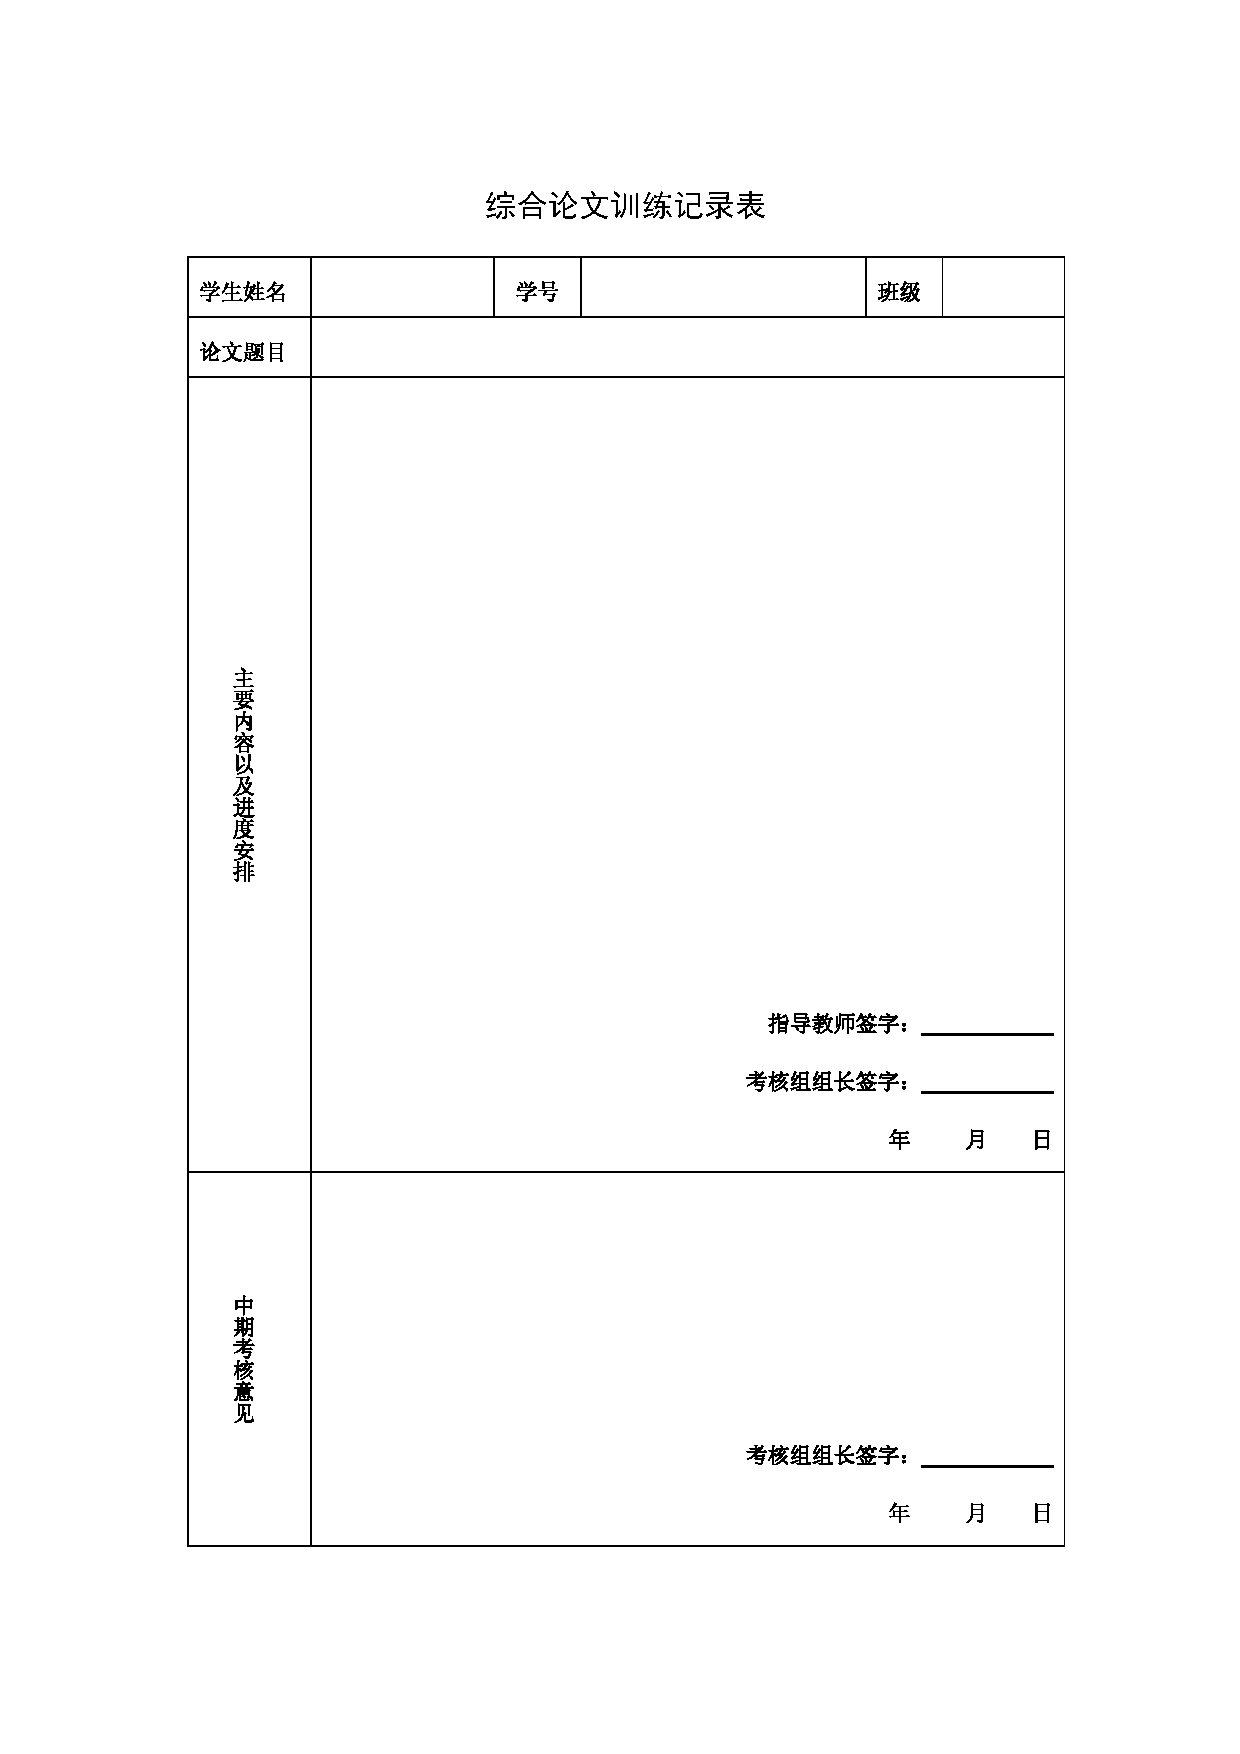
\includepdf[pages=-]{scan-record.pdf}
\end{document}
